% !TeX program = xelatex
% !TeX encoding = UTF-8
% Biên soạn bằng XeLaTeX. Chạy XeLaTeX ít nhất hai lần để cập nhật mục lục và liên kết chéo.

\documentclass[12pt,a4paper]{article}

% ============================================================
% Gói lệnh và định dạng chung
% ============================================================
\usepackage{fontspec}
\usepackage{unicode-math}

% Ưu tiên Times New Roman và Cambria Math trên Windows/TeXStudio.
% Các phông dự phòng giúp tệp vẫn biên soạn được trên hệ thống không có phông Microsoft.
\IfFontExistsTF{Times New Roman}{%
  \setmainfont{Times New Roman}
}{%
  \setmainfont{Liberation Serif}
}
\setsansfont{LibertinusSans-Regular.otf}[
  BoldFont=LibertinusSans-Bold.otf,
  ItalicFont=LibertinusSans-Italic.otf
]
\setmonofont{LibertinusMono-Regular.otf}
\IfFontExistsTF{Cambria Math}{%
  \setmathfont{Cambria Math}
}{%
  \setmathfont{LibertinusMath-Regular.otf}
}

\usepackage[a4paper,top=2.4cm,bottom=2.4cm,left=2.8cm,right=2.4cm]{geometry}
\usepackage{setspace}
\onehalfspacing
\usepackage{microtype}
\usepackage{indentfirst}
\setlength{\parindent}{1.2cm}
\setlength{\parskip}{0.15em}
\setlength{\emergencystretch}{3em}

\usepackage{amsthm}
\numberwithin{equation}{section}

\usepackage{graphicx}
\usepackage{tikz}
\usetikzlibrary{calc}
\usepackage{float}
\usepackage{caption}
\usepackage{subcaption}
\usepackage{booktabs}
\usepackage{longtable}
\usepackage{tabularx}
\usepackage{array}
\usepackage{multirow}
\usepackage{threeparttable}
\usepackage{makecell}
\usepackage{pdflscape}

\usepackage{enumitem}
\setlist[itemize]{leftmargin=1.7em,itemsep=0.25em,topsep=0.35em}
\setlist[enumerate]{leftmargin=2.0em,itemsep=0.25em,topsep=0.35em}

\usepackage[dvipsnames,table]{xcolor}
\definecolor{LinkBlue}{RGB}{22,70,120}
\definecolor{CiteGreen}{RGB}{20,95,65}
\definecolor{PlaceholderRed}{RGB}{150,35,35}
\definecolor{LightGray}{RGB}{245,246,248}
\definecolor{CoverNavy}{RGB}{24,45,68}
\definecolor{CoverBlue}{RGB}{45,82,118}
\definecolor{CoverRule}{RGB}{160,169,178}
\definecolor{JournalGray}{RGB}{92,99,106}

\usepackage{xurl}
\usepackage{hyperref}
\hypersetup{
  unicode=true,
  colorlinks=true,
  linkcolor=LinkBlue,
  citecolor=CiteGreen,
  urlcolor=LinkBlue,
  pdfauthor={Nguyễn Hoài Nam; Nguyễn Thuận Hiếu; Đặng Chí Hiếu},
  pdftitle={Ước lượng và dự báo biến động theo trạng thái thị trường bằng mô hình MS-GARCH-X với sai số Student-t},
  pdfsubject={MS-GARCH-X, Student-t, MLE, Variational Bayes, MCMC, VN30F1M},
  pdfkeywords={MS-GARCH-X, Student-t, MLE, Variational Bayes, MCMC, VN30F1M, VaR}
}
\usepackage{bookmark}
\usepackage[nameinlink,noabbrev]{cleveref}

\crefname{section}{Mục}{Các mục}
\Crefname{section}{Mục}{Các mục}
\crefname{subsection}{tiểu mục}{các tiểu mục}
\Crefname{subsection}{Tiểu mục}{Các tiểu mục}
\crefname{equation}{phương trình}{các phương trình}
\Crefname{equation}{Phương trình}{Các phương trình}
\crefname{figure}{hình}{các hình}
\Crefname{figure}{Hình}{Các hình}
\crefname{table}{bảng}{các bảng}
\Crefname{table}{Bảng}{Các bảng}
\crefname{appendix}{phụ lục}{các phụ lục}
\Crefname{appendix}{Phụ lục}{Các phụ lục}

\usepackage{fancyhdr}
\setlength{\headheight}{16pt}

% Kiểu trang dành cho phần nội dung chính của bài báo.
\fancypagestyle{mainpaper}{%
  \fancyhf{}
  \fancyhead[L]{\footnotesize\itshape Nguyễn Hoài Nam, Nguyễn Thuận Hiếu, Đặng Chí Hiếu}
  \fancyhead[R]{\footnotesize\itshape MS-GARCH-X Student-t cho VN30F1M}
  \fancyfoot[L]{\footnotesize\color{JournalGray} Nghiên cứu khoa học sinh viên \NienKhoa}
  \fancyfoot[C]{\footnotesize \thepage}
  \fancyfoot[R]{\footnotesize\color{JournalGray} \NgayBanThao}
  \renewcommand{\headrulewidth}{0.4pt}
  \renewcommand{\footrulewidth}{0.3pt}
}

% Kiểu trang tối giản cho phần đầu: tóm tắt, mục lục và danh mục.
\fancypagestyle{preliminary}{%
  \fancyhf{}
  \fancyfoot[C]{\footnotesize \thepage}
  \renewcommand{\headrulewidth}{0pt}
  \renewcommand{\footrulewidth}{0pt}
}
\pagestyle{preliminary}

\usepackage{titlesec}
\titleformat{\section}{\Large\bfseries}{\thesection.}{0.65em}{}
\titleformat{\subsection}{\large\bfseries}{\thesubsection.}{0.55em}{}
\titleformat{\subsubsection}{\normalsize\bfseries}{\thesubsubsection.}{0.5em}{}
\titlespacing*{\section}{0pt}{1.3em}{0.7em}
\titlespacing*{\subsection}{0pt}{1.0em}{0.5em}

\renewcommand{\contentsname}{Mục lục}
\renewcommand{\listfigurename}{Danh mục hình}
\renewcommand{\listtablename}{Danh mục bảng}
\renewcommand{\figurename}{Hình}
\renewcommand{\tablename}{Bảng}
\renewcommand{\refname}{Tài liệu tham khảo}
\renewcommand{\appendixname}{Phụ lục}

% ============================================================
% Môi trường và lệnh tùy chỉnh
% ============================================================
\newtheorem{definition}{Định nghĩa}[section]
\newtheorem{proposition}{Mệnh đề}[section]
\newtheorem{remark}{Nhận xét}[section]

\newcommand{\bm}[1]{\symbf{#1}}
\newcommand{\Data}{\mathcal{D}}
\newcommand{\Info}{\mathcal{F}}
\newcommand{\Param}{\bm{\theta}}
\newcommand{\Xvec}{\bm{X}}
\newcommand{\Pmat}{\bm{P}}
\newcommand{\R}{\mathbb{R}}
\newcommand{\E}{\mathbb{E}}
\newcommand{\Var}{\operatorname{Var}}
\newcommand{\Cov}{\operatorname{Cov}}
\newcommand{\Prob}{\mathbb{P}}
\newcommand{\diag}{\operatorname{diag}}
\newcommand{\softplus}{\operatorname{softplus}}
\newcommand{\VaR}{\operatorname{VaR}}
\newcommand{\ES}{\operatorname{ES}}
\newcommand{\RMSE}{\operatorname{RMSE}}
\newcommand{\MAE}{\operatorname{MAE}}
\newcommand{\QLIKE}{\operatorname{QLIKE}}
\newcommand{\CRPS}{\operatorname{CRPS}}
\newcommand{\ELBO}{\operatorname{ELBO}}
\newcommand{\KL}{\operatorname{KL}}
\newcommand{\ESS}{\operatorname{ESS}}
\newcommand{\AIC}{\operatorname{AIC}}
\newcommand{\BIC}{\operatorname{BIC}}
\newcommand{\ind}{\mathbb{I}}
\newcommand{\doi}[1]{\href{https://doi.org/#1}{\nolinkurl{#1}}}
\newcommand{\CanBoSung}[1]{\textcolor{PlaceholderRed}{\textbf{[Cần bổ sung: #1]}}}
\newcommand{\KhongCoSoLieu}{\multicolumn{1}{c}{--}}
\newcommand{\RQ}[1]{\textbf{RQ#1}}

\newcolumntype{Y}{>{\raggedright\arraybackslash}X}
\newcolumntype{C}{>{\centering\arraybackslash}X}
\newcolumntype{R}{>{\raggedleft\arraybackslash}X}

\captionsetup{font=small,labelfont=bf,labelsep=period}

% ============================================================
% Thông tin nhóm nghiên cứu và trang bìa
% ============================================================
\newcommand{\TacGiaMot}{Nguyễn Hoài Nam}
\newcommand{\MSSVMot}{C2300152}
\newcommand{\EmailMot}{C2300152@student.tdtu.edu.vn}
\newcommand{\TacGiaHai}{Nguyễn Thuận Hiếu}
\newcommand{\MSSVHai}{C2300128}
\newcommand{\EmailHai}{c2300128@student.tdtu.edu.vn}
\newcommand{\TacGiaBa}{Đặng Chí Hiếu}
\newcommand{\MSSVBa}{C2400097}
\newcommand{\EmailBa}{c2400097@student.tdtu.edu.vn}
\newcommand{\TenTacGia}{\TacGiaMot, \TacGiaHai, \TacGiaBa}
\newcommand{\DonViCongTac}{Khoa Toán -- Thống kê, Trường Đại học Tôn Đức Thắng}
\newcommand{\ThuDienTu}{\EmailMot}
\newcommand{\NgayBanThao}{Tháng 7 năm 2026}
\newcommand{\TenTruong}{TỔNG LIÊN ĐOÀN LAO ĐỘNG VIỆT NAM}
\newcommand{\TenKhoa}{TRƯỜNG ĐẠI HỌC TÔN ĐỨC THẮNG}
\newcommand{\NienKhoa}{2025--2026}
\newcommand{\GiangVienHuongDan}{TS. Trương Bửu Châu}
\newcommand{\NoiVaThoiGian}{TP. Hồ Chí Minh, tháng 7 năm 2026}
\newcommand{\TieuDeViet}{Ước lượng và dự báo biến động theo \\ trạng thái thị trường với mô hình MS-GARCH-X với sai số Student-t}
\newcommand{\TieuDePhu}{Sử dụng các phương pháp MLE, Variational Bayes và MCMC trên thị trường hợp đồng tương lai VN30}
\newcommand{\TieuDeDayDu}{\TieuDeViet: \TieuDePhu}
\newcommand{\TieuDeAnh}{Regime-Switching Volatility Estimation and Forecasting with a Student-t MS-GARCH-X Model: A Comparison of Maximum Likelihood, Variational Bayes, and Markov Chain Monte Carlo in the VN30 Index Futures Market}

\begin{document}

% ============================================================
% Trang bìa thứ nhất: bản nộp tại Trường Đại học Tôn Đức Thắng
% ============================================================
\begin{titlepage}
    \thispagestyle{empty}

    \begin{tikzpicture}[remember picture,overlay]
        \draw[line width=1.6pt]
        ($(current page.north west)+(2.35cm,-1.65cm)$)
        rectangle
        ($(current page.south east)+(-1.65cm,1.65cm)$);
        \draw[line width=0.45pt]
        ($(current page.north west)+(2.48cm,-1.78cm)$)
        rectangle
        ($(current page.south east)+(-1.78cm,1.78cm)$);
    \end{tikzpicture}

    \centering
    \vspace*{0.10cm}
    {\fontsize{15pt}{18pt}\selectfont\bfseries \TenTruong\par}
    \vspace{0.12cm}
    {\fontsize{15pt}{18pt}\selectfont\bfseries \TenKhoa\par}

    \vspace{1.10cm}
    
\includegraphics[width=0.31\textwidth]{logo.png}

    \vspace{0.90cm}
    {\fontsize{21pt}{25pt}\selectfont\bfseries CÔNG TRÌNH NGHIÊN CỨU KHOA HỌC SINH VIÊN \NienKhoa\par}

    \vspace{0.70cm}
    \begin{minipage}{0.78\textwidth}
        \centering
        {\fontsize{16.5pt}{21pt}\selectfont\bfseries \TieuDeDayDu\par}
    \end{minipage}

    \vspace{0.85cm}
    \renewcommand{\arraystretch}{1.45}
    \setlength{\tabcolsep}{7pt}
    \begin{tabularx}{0.80\textwidth}{|>{\bfseries}p{0.23\textwidth}|X|>{\centering\arraybackslash}p{0.16\textwidth}|}
        \hline
        Năm học & \multicolumn{2}{l|}{\NienKhoa} \\
        \hline
        Đơn vị & \multicolumn{2}{l|}{Khoa Toán-Thống kê} \\
        \hline
        \multirow{3}{*}{\makecell[l]{Nhóm nghiên cứu}}
        & \TacGiaMot & \MSSVMot \\
        \cline{2-3}
        & \TacGiaHai & \MSSVHai \\
        \cline{2-3}
        & \TacGiaBa & \MSSVBa \\
        \hline
        \makecell[l]{Giảng viên\\hướng dẫn}
        & \multicolumn{2}{l|}{\GiangVienHuongDan} \\
        \hline
    \end{tabularx}

    \vfill
    {\fontsize{12pt}{15pt}\selectfont\bfseries \MakeUppercase{\NoiVaThoiGian}\par}
    \vspace{0.55cm}
\end{titlepage}

% ============================================================
% Trang bìa thứ hai: trang tiêu đề học thuật của bài báo
% ============================================================
\begin{titlepage}
    \thispagestyle{empty}

    \vspace*{0.35cm}
    \noindent
    \begin{minipage}[t]{0.64\textwidth}
        {\small\bfseries\color{CoverNavy} NGHIÊN CỨU KHOA HỌC SINH VIÊN}\par
        {\footnotesize\color{JournalGray} Trường Đại học Tôn Đức Thắng}
    \end{minipage}
    \begin{minipage}[t]{0.35\textwidth}
        \raggedleft
        {\footnotesize\color{JournalGray} \NgayBanThao}\par
        {\footnotesize\color{JournalGray} TP. Hồ Chí Minh}
    \end{minipage}

    \vspace{0.35cm}
    \par\noindent{\color{CoverNavy}\rule{\linewidth}{1.1pt}}

    \vspace{1.20cm}
    \begin{center}
        \begin{minipage}{0.92\textwidth}
            \centering
            {\fontsize{22pt}{28pt}\selectfont\bfseries\color{CoverNavy} \TieuDeDayDu\par}
            \vspace{0.70cm}
            {\fontsize{13.5pt}{18pt}\selectfont\itshape \TieuDeAnh\par}
        \end{minipage}
    \end{center}

    \vspace{1.25cm}
    \begin{center}
        {\fontsize{14pt}{18pt}\selectfont\bfseries
        \TacGiaMot\textsuperscript{1,*},
        \TacGiaHai\textsuperscript{1},
        \TacGiaBa\textsuperscript{1}}\par

        \vspace{0.42cm}
        {\small\textsuperscript{1}\DonViCongTac}\par
        \vspace{0.50cm}
        \begin{tabular}{@{}r@{\ }l@{}}
            \TacGiaMot: & \href{mailto:\EmailMot}{\nolinkurl{\EmailMot}} \\
            \TacGiaHai: & \href{mailto:\EmailHai}{\nolinkurl{\EmailHai}} \\
            \TacGiaBa: & \href{mailto:\EmailBa}{\nolinkurl{\EmailBa}} \\
        \end{tabular}
    \end{center}

    \vspace{1.15cm}
    \par\noindent{\color{CoverRule}\rule{\linewidth}{0.5pt}}
    \vspace{0.45cm}

    \noindent\begin{minipage}{\linewidth}
        \small
        \textbf{Tác giả liên hệ:} \TacGiaBa,
        \href{mailto:\EmailBa}{\nolinkurl{\EmailBa}}.\\[0.35em]
        \textbf{Hướng dẫn khoa học:} Nghiên cứu được thực hiện dưới sự hướng dẫn của \GiangVienHuongDan. 
    \end{minipage}

    \vfill
    \noindent{\color{CoverNavy}\rule{\linewidth}{1pt}}
    \vspace{0.15cm}

    \noindent
\end{titlepage}


% ============================================================
% Tóm tắt
% ============================================================
\pagestyle{preliminary}
\pagenumbering{roman}
\setcounter{page}{1}

\begin{abstract}
Biến động lợi suất trên thị trường hợp đồng tương lai thường biểu hiện tính tập trung theo cụm, đuôi phân phối dày và sự thay đổi cấu trúc theo thời gian. Những đặc điểm này làm suy giảm tính phù hợp của mô hình GARCH một trạng thái với giả định sai số chuẩn, đặc biệt khi mục tiêu nghiên cứu bao gồm dự báo mật độ và đo lường rủi ro đuôi. Bài báo xây dựng một khung MS-GARCH-X với sai số Student-t cho lợi suất hợp đồng tương lai VN30F1M. Trong mô hình đề xuất, trạng thái biến động thấp và trạng thái biến động cao được điều khiển bởi một chuỗi Markov ẩn; các biến ngoại sinh có thể bao gồm thanh khoản, biến động thực tế, chênh lệch giá hợp đồng tương lai so với chỉ số cơ sở, ngày đáo hạn và thời điểm chuyển hợp đồng. Ba phương pháp ước lượng và suy diễn được so sánh trên cùng một cấu trúc mô hình: ước lượng hợp lý cực đại, Variational Bayes và Markov Chain Monte Carlo. Khung đánh giá bao gồm độ chính xác ước lượng trong nghiên cứu mô phỏng, chất lượng dự báo biến động ngoài mẫu, dự báo mật độ, kiểm định VaR, độ hiệu chỉnh xác suất trạng thái và chi phí tính toán. Bài báo đồng thời xem xét vai trò của việc truyền bất định tham số vào phân phối dự báo và phân tích khả năng bậc tự do của phân phối Student-t thay đổi theo trạng thái. Các kết quả định lượng sẽ được cập nhật sau khi quy trình dữ liệu và thực nghiệm được hoàn tất.

\vspace{0.6em}
\noindent\textbf{Từ khóa:} biến động có điều kiện; MS-GARCH-X; phân phối Student-t; Variational Bayes; Markov Chain Monte Carlo; hợp đồng tương lai VN30; VaR.
\end{abstract}

\newpage
\tableofcontents
\newpage
\listoftables
\newpage
\listoffigures
\newpage

% ============================================================
% Danh mục ký hiệu
% ============================================================
\section*{Danh mục ký hiệu}
\addcontentsline{toc}{section}{Danh mục ký hiệu}

\begin{longtable}{>{\centering\arraybackslash}p{0.18\textwidth}p{0.72\textwidth}}
\toprule
\textbf{Ký hiệu} & \textbf{Diễn giải} \\
\midrule
\endfirsthead
\toprule
\textbf{Ký hiệu} & \textbf{Diễn giải} \\
\midrule
\endhead
$P_t$ & Giá đóng cửa hoặc giá đại diện của hợp đồng tương lai tại thời điểm $t$. \\
$r_t$ & Lợi suất logarit tại thời điểm $t$. \\
$S_t$ & Trạng thái ẩn tại thời điểm $t$, với $S_t\in\{1,2\}$. \\
$\Info_t$ & Tập thông tin quan sát được đến hết thời điểm $t$. \\
$\Data_T$ & Toàn bộ dữ liệu dùng cho suy diễn đến thời điểm $T$. \\
$\mu_s$ & Trung bình có điều kiện của lợi suất trong trạng thái $s$. \\
$\varepsilon_t$ & Nhiễu của phương trình trung bình tại thời điểm $t$. \\
$h_{t,s}$ & Phương sai có điều kiện tại thời điểm $t$ khi $S_t=s$. \\
$z_t$ & Sai số chuẩn hóa có kỳ vọng bằng $0$ và phương sai bằng $1$. \\
$\nu$ & Bậc tự do chung của phân phối Student-t chuẩn hóa. \\
$\nu_s$ & Bậc tự do riêng của trạng thái $s$ trong mô hình mở rộng. \\
$\omega_s,\alpha_s,\beta_s$ & Các hệ số phương sai có điều kiện của trạng thái $s$. \\
$\bm{\gamma}_s$ & Vector hệ số của các biến ngoại sinh trong trạng thái $s$. \\
$\Xvec_{t-1}$ & Vector biến ngoại sinh đã biết tại thời điểm lập dự báo. \\
$p_{ij}$ & Xác suất chuyển từ trạng thái $i$ tại $t-1$ sang trạng thái $j$ tại $t$. \\
$\Pmat$ & Ma trận chuyển trạng thái Markov. \\
$\xi_{t\mid u}(s)$ & Xác suất $S_t=s$ có điều kiện trên thông tin đến thời điểm $u$. \\
$\Param$ & Vector chứa toàn bộ tham số liên tục của mô hình. \\
$q(\Param)$ & Phân phối xấp xỉ hậu nghiệm trong Variational Bayes. \\
$RV_t$ & Biến động thực tế tại ngày $t$, được xây dựng từ lợi suất nội ngày. \\
$\VaR_{t,\alpha}$ & Giá trị rủi ro tại mức xác suất đuôi $\alpha$. \\
$\widehat R$ & Chỉ số chẩn đoán hội tụ giữa các chuỗi MCMC. \\
$\ESS$ & Cỡ mẫu hiệu dụng của chuỗi MCMC. \\
\bottomrule
\end{longtable}

\clearpage
\pagenumbering{arabic}
\setcounter{page}{1}
\pagestyle{mainpaper}

% ============================================================
\section{Giới thiệu}\label{sec:gioi-thieu}
% ============================================================

\subsection{Bối cảnh nghiên cứu}\label{subsec:boi-canh}

Biến động là một đại lượng trung tâm trong kinh tế lượng tài chính vì nó chi phối trực tiếp mức độ bất định của lợi suất, yêu cầu ký quỹ, định giá tài sản phái sinh và giới hạn rủi ro của danh mục. Khác với giả định phương sai không đổi trong mô hình hồi quy tuyến tính cổ điển, chuỗi lợi suất tài chính thường xuất hiện các giai đoạn yên ổn xen kẽ với các giai đoạn biến động mạnh. Hiện tượng các quan sát có độ lớn tương tự xuất hiện gần nhau theo thời gian được gọi là tính tập trung theo cụm của biến động. Mô hình ARCH của \cite{engle1982} và mô hình GARCH của \cite{bollerslev1986} được phát triển nhằm mô tả đặc điểm này thông qua phương sai có điều kiện biến đổi theo thời gian.

Bên cạnh tính tập trung theo cụm, lợi suất tài chính thường có nhiều quan sát cực đoan hơn mức được dự đoán bởi phân phối chuẩn. Khi mô hình giả định sai số chuẩn trong khi dữ liệu có đuôi dày, xác suất của các khoản lỗ lớn có thể bị đánh giá thấp. Phân phối Student-t là một lựa chọn phổ biến vì tham số bậc tự do cho phép điều chỉnh trực tiếp độ dày của đuôi phân phối \cite{bollerslev1987}.

Một hạn chế khác của mô hình GARCH một trạng thái là giả định toàn bộ mẫu dữ liệu được tạo ra bởi một cơ chế biến động duy nhất. Trên thực tế, phản ứng của thị trường đối với thông tin mới, mức độ dai dẳng của biến động và xác suất xuất hiện các biến cố cực đoan có thể khác nhau giữa giai đoạn bình thường và giai đoạn căng thẳng. Mô hình chuyển trạng thái Markov cho phép các tham số thay đổi theo một trạng thái ẩn, trong đó trạng thái hiện tại phụ thuộc xác suất vào trạng thái liền trước \cite{hamilton1989}. Khi kết hợp chuỗi Markov với phương trình GARCH, mô hình có thể mô tả đồng thời tính dai dẳng bên trong từng trạng thái và sự chuyển đổi giữa các chế độ biến động \cite{gray1996,klaassen2002,haas2004}.

Đối với hợp đồng tương lai VN30F1M, biến động có thể chịu tác động của thanh khoản, biến động quan sát trong ngày, chênh lệch giữa giá hợp đồng tương lai và chỉ số cơ sở, ngày đáo hạn và quá trình chuyển sang hợp đồng kế tiếp. Việc đưa các đại lượng này vào phương trình phương sai tạo thành cấu trúc GARCH-X. Ký hiệu ``X'' nhấn mạnh rằng ngoài thành phần ARCH và GARCH, phương sai có điều kiện còn phụ thuộc vào một vector biến ngoại sinh được xác định trước thời điểm dự báo. Mức độ mà mỗi biến này thực sự được đưa vào mô hình chính phụ thuộc vào khả năng tiếp cận dữ liệu tương ứng; \cref{subsec:exogenous-variables} trình bày cụ thể tập biến khả dụng với nguồn dữ liệu hiện có của nghiên cứu.

Nghiên cứu này tập trung vào hai nhóm bất định. Nhóm thứ nhất là bất định ngẫu nhiên của lợi suất tương lai ngay cả khi biết tham số mô hình. Nhóm thứ hai là bất định nhận thức do tham số, trạng thái và cấu trúc mô hình chưa được biết chính xác. Ước lượng hợp lý cực đại cung cấp một nghiệm ước lượng điểm và thường dựa vào xấp xỉ tiệm cận để xây dựng sai số chuẩn. Ngược lại, suy diễn Bayes biểu diễn bất định tham số bằng phân phối hậu nghiệm. MCMC có thể mô tả hậu nghiệm tương đối linh hoạt nhưng thường tốn thời gian tính toán, trong khi Variational Bayes chuyển bài toán tích phân thành một bài toán tối ưu và thường nhanh hơn \cite{jordan1999,blei2017}.

\subsection{Vấn đề nghiên cứu}\label{subsec:van-de}

Bài báo xem xét đồng thời sáu hạn chế thường gặp trong mô hình hóa biến động. Thứ nhất, giả định chuẩn có thể không phù hợp với lợi suất có đuôi dày. Thứ hai, mô hình một trạng thái không phản ánh được thay đổi cấu trúc. Thứ ba, mô hình không có biến ngoại sinh có thể bỏ qua thông tin quan sát được có liên hệ với biến động. Thứ tư, ước lượng điểm không thể hiện đầy đủ bất định của tham số. Thứ năm, các phương pháp suy diễn hậu nghiệm khác nhau có thể tạo ra mức đánh đổi khác nhau giữa độ chính xác và chi phí tính toán. Thứ sáu, việc đánh giá mô hình chỉ bằng độ phù hợp trong mẫu không bảo đảm chất lượng dự báo mật độ hoặc rủi ro đuôi ngoài mẫu.

Từ các hạn chế trên, vấn đề nghiên cứu được phát biểu như sau: liệu một mô hình MS-GARCH-X với sai số Student-t có mô tả và dự báo tốt hơn cấu trúc biến động của VN30F1M so với các mô hình một trạng thái; và trong cùng một cấu trúc mô hình, MLE, Variational Bayes và MCMC khác nhau như thế nào về ước lượng tham số, bất định hậu nghiệm, xác suất trạng thái, dự báo biến động, dự báo mật độ, kiểm định VaR và thời gian tính toán?

\subsection{Mục tiêu nghiên cứu}\label{subsec:muc-tieu}

Mục tiêu tổng quát của bài báo là xây dựng mô hình MS-GARCH-X Student-t cho lợi suất hợp đồng tương lai VN30F1M và so sánh MLE, Variational Bayes và MCMC trên một thiết kế thực nghiệm thống nhất.

Các mục tiêu cụ thể bao gồm:
\begin{enumerate}
  \item mô tả đặc điểm thống kê của lợi suất VN30F1M, bao gồm tính dừng, tự tương quan, hiệu ứng ARCH và độ dày của đuôi phân phối;
  \item xây dựng mô hình GARCH-X và MS-GARCH-X với phân phối chuẩn và Student-t chuẩn hóa;
  \item ước lượng mô hình MS-GARCH-X Student-t bằng MLE, Variational Bayes và MCMC trong cùng điều kiện dữ liệu và cùng quy trình dự báo;
  \item đánh giá độ chính xác ước lượng trên dữ liệu mô phỏng, nơi tham số thật và trạng thái thật được biết trước;
  \item đánh giá chất lượng dự báo ngoài mẫu bằng các hàm mất mát biến động, điểm số dự báo mật độ và kiểm định VaR;
  \item lượng hóa chi phí tính toán, độ ổn định và chẩn đoán hội tụ của từng phương pháp;
  \item kiểm tra trong mô hình mở rộng liệu trạng thái biến động cao có đuôi phân phối dày hơn trạng thái biến động thấp hay không.
\end{enumerate}

\subsection{Câu hỏi nghiên cứu}\label{subsec:cau-hoi}

Bài báo được tổ chức quanh sáu câu hỏi nghiên cứu sau:

\begin{description}[style=nextline,leftmargin=1.7cm,labelwidth=1.3cm]
  \item[\RQ{1}.] Phân phối Student-t có cải thiện độ phù hợp và chất lượng dự báo lợi suất VN30F1M so với phân phối chuẩn hay không?
  \item[\RQ{2}.] MS-GARCH-X có cải thiện dự báo biến động và rủi ro so với GARCH-X một trạng thái hay không?
  \item[\RQ{3}.] Variational Bayes có thể xấp xỉ phân phối hậu nghiệm của MS-GARCH-X Student-t đủ gần với MCMC hay không?
  \item[\RQ{4}.] Việc tích hợp bất định tham số vào phân phối dự báo có cải thiện dự báo mật độ và độ hiệu chỉnh VaR hay không?
  \item[\RQ{5}.] Mức đánh đổi giữa độ chính xác, độ tin cậy và thời gian tính toán của MLE, Variational Bayes và MCMC là gì?
  \item[\RQ{6}.] Mức độ đuôi dày có khác nhau giữa trạng thái biến động thấp và trạng thái biến động cao hay không?
\end{description}

Câu hỏi \RQ{6} chỉ được kiểm tra trực tiếp trong mô hình mở rộng có bậc tự do riêng theo trạng thái. Khi trạng thái $1$ được nhận dạng là trạng thái biến động thấp và trạng thái $2$ là trạng thái biến động cao, đại lượng hậu nghiệm cần quan tâm là
\begin{equation}
  \Prob\!\left(\nu_{2}<\nu_{1}\mid\Data_T\right).
  \label{eq:tail-probability}
\end{equation}
Nếu xác suất trong \cref{eq:tail-probability} gần $1$, dữ liệu cung cấp bằng chứng rằng trạng thái biến động cao có đuôi dày hơn. Mô hình chính sử dụng một bậc tự do chung $\nu$ để hạn chế số tham số và giảm rủi ro nhận dạng yếu; mô hình có $\nu_s$ riêng được đặt trong phần kiểm định độ bền.

\subsection{Đóng góp của nghiên cứu}\label{subsec:dong-gop}

Bài báo dự kiến đóng góp theo năm hướng. Thứ nhất, nghiên cứu xây dựng một khung MS-GARCH-X Student-t dành cho chuỗi hợp đồng tương lai VN30F1M, đồng thời trình bày minh bạch vấn đề tạo chuỗi hợp đồng liên tục và chỉ rõ giới hạn cụ thể của nguồn dữ liệu hiện có đối với việc xây dựng chuỗi này (\cref{subsec:continuous-contract}), làm cơ sở cho hướng mở rộng khi có dữ liệu tách theo từng hợp đồng thành phần. Thứ hai, ba phương pháp MLE, Variational Bayes và MCMC được so sánh trên cùng một hàm hợp lý và cùng cấu trúc mô hình, qua đó hạn chế việc quy kết sai khác kết quả cho những đặc tả không đồng nhất. Thứ ba, việc đánh giá không dừng ở dự báo điểm mà mở rộng sang dự báo mật độ, VaR và độ hiệu chỉnh xác suất trạng thái. Thứ tư, nghiên cứu mô phỏng được sử dụng để đánh giá sai lệch, RMSE và xác suất bao phủ khi tham số thật được biết. Thứ năm, nghiên cứu lượng hóa mức đánh đổi giữa chất lượng suy diễn và chi phí tính toán, một yếu tố quan trọng khi mô hình cần tái ước lượng định kỳ.

\subsection{Cấu trúc bài báo}\label{subsec:cau-truc}

Phần còn lại của bài báo được tổ chức như sau. \Cref{sec:tong-quan} tổng hợp các hướng nghiên cứu liên quan và xác định khoảng trống. \Cref{sec:ly-thuyet} trình bày cơ sở lý thuyết và đặc tả mô hình. \Cref{sec:suy-dien} mô tả hàm hợp lý, MLE, suy diễn Bayes, Variational Bayes, MCMC và dự báo hậu nghiệm. \Cref{sec:du-lieu} trình bày dữ liệu và thiết kế thực nghiệm. \Cref{sec:kiem-dinh} mô tả các kiểm định thống kê ban đầu. \Cref{sec:mo-phong} xây dựng nghiên cứu mô phỏng. \Cref{sec:ket-qua} cung cấp khung báo cáo kết quả. \Cref{sec:thao-luan} thảo luận cách diễn giải kết quả. \Cref{sec:han-che} trình bày hạn chế và định hướng nghiên cứu. \Cref{sec:ket-luan} kết luận bài báo.

% ============================================================
\section{Tổng quan tài liệu}\label{sec:tong-quan}
% ============================================================

\subsection{Từ ARCH đến GARCH}\label{subsec:arch-garch-review}

Mô hình ARCH của \cite{engle1982} xuất phát từ nhận xét rằng phương sai của nhiễu có thể phụ thuộc vào bình phương các cú sốc quá khứ. Mô hình này tạo nền tảng cho một lớp mô hình phương sai có điều kiện, trong đó động lực của biến động được mô hình hóa trực tiếp thay vì xem phương sai là hằng số. Tuy nhiên, để mô tả tính dai dẳng cao, ARCH thường cần nhiều độ trễ và do đó làm tăng số tham số.

Mô hình GARCH của \cite{bollerslev1986} bổ sung các độ trễ của chính phương sai có điều kiện. Đặc tả GARCH$(1,1)$ với số tham số nhỏ có thể tạo ra quá trình biến động dai dẳng và trở thành một chuẩn đối chứng phổ biến. Trong các ứng dụng tài chính, mô hình GARCH được dùng để dự báo biến động, xây dựng phân phối lợi suất có điều kiện, tính VaR và hỗ trợ định giá tài sản phái sinh.

\subsection{Phân phối sai số trong mô hình GARCH}\label{subsec:dist-review}

Giả định chuẩn thuận lợi cho suy luận nhưng thường không mô tả đầy đủ độ nhọn và đuôi dày của lợi suất. \cite{bollerslev1987} đưa phân phối Student-t có điều kiện vào mô hình biến động, cho phép các quan sát cực đoan có xác suất lớn hơn so với phân phối chuẩn. Khi bậc tự do $\nu$ tăng, phân phối Student-t tiến gần phân phối chuẩn; khi $\nu$ giảm nhưng vẫn lớn hơn $2$, đuôi trở nên dày hơn trong khi phương sai vẫn hữu hạn.

Các mở rộng khác bao gồm phân phối Student-t lệch và các phân phối linh hoạt hơn. Tuy nhiên, tăng tính linh hoạt cũng làm tăng rủi ro nhận dạng yếu, tương quan hậu nghiệm mạnh và khó hội tụ. Vì vậy, nghiên cứu này sử dụng Student-t đối xứng làm mô hình chính, sau đó xem phân phối lệch là một hướng kiểm định độ bền hoặc nghiên cứu tiếp theo.

\subsection{Mô hình GARCH-X}\label{subsec:garchx-review}

GARCH-X mở rộng phương trình phương sai bằng cách đưa thêm các biến quan sát được. Về mặt kinh tế, các biến này đại diện cho thông tin có thể giải thích biến động ngoài bình phương cú sốc và phương sai trễ. Đối với hợp đồng tương lai, những ứng viên có cơ sở bao gồm khối lượng giao dịch, biến động thực tế trễ, chênh lệch giá hợp đồng tương lai so với chỉ số cơ sở, biến giả ngày đáo hạn và biến giả chuyển hợp đồng.

Một yêu cầu quan trọng là các biến ngoại sinh phải khả dụng tại thời điểm dự báo. Việc sử dụng biến được tính từ toàn bộ ngày $t$ để dự báo chính ngày $t$ tạo ra sai lệch nhìn trước. Do đó, nghiên cứu này ưu tiên $\Xvec_{t-1}$ hoặc các biến lịch đã biết trước, chẳng hạn biến giả ngày đáo hạn tại $t$.

\subsection{Mô hình Markov-switching GARCH}\label{subsec:msgarch-review}

Mô hình chuyển trạng thái của \cite{hamilton1989} cho phép tham số thay đổi theo một chuỗi Markov ẩn. Khi áp dụng vào GARCH, mỗi trạng thái có thể có mức biến động nền, độ nhạy với cú sốc và độ dai dẳng khác nhau. \cite{gray1996} đề xuất cơ chế thu gọn để xử lý sự phụ thuộc của phương sai vào toàn bộ đường đi trạng thái. \cite{klaassen2002} phát triển một đặc tả cho phép dự báo nhiều bước thuận tiện hơn. \cite{haas2004} đề xuất một cách tiếp cận khác nhằm khắc phục một số khó khăn của MS-GARCH truyền thống.

Khó khăn cốt lõi của MS-GARCH là phương sai tại thời điểm $t$ phụ thuộc vào trạng thái hiện tại và phương sai ở $t-1$, trong khi phương sai ở $t-1$ lại phụ thuộc vào trạng thái trước đó. Nếu giữ toàn bộ lịch sử trạng thái, số đường đi tăng theo cấp số nhân. Các phương pháp thu gọn thay thế hỗn hợp đường đi bằng một hoặc một số moment có điều kiện, qua đó giữ được tính đệ quy của hàm hợp lý.

\subsection{MLE, Variational Bayes và MCMC}\label{subsec:inference-review}

MLE xác định tham số bằng cách cực đại hóa hàm hợp lý. Ưu điểm chính là quy trình tương đối trực tiếp, dễ so sánh bằng AIC hoặc BIC và thường nhanh hơn suy diễn Bayes đầy đủ. Hạn chế là sai số chuẩn dựa vào xấp xỉ cục bộ có thể không phản ánh tốt hậu nghiệm lệch, đa đỉnh hoặc có tương quan mạnh.

Suy diễn Bayes kết hợp hàm hợp lý với phân phối tiền nghiệm để tạo phân phối hậu nghiệm. MCMC xấp xỉ các kỳ vọng hậu nghiệm bằng mẫu từ một chuỗi Markov có phân phối dừng là hậu nghiệm mục tiêu. Các thuật toán nền tảng gồm Metropolis--Hastings \cite{metropolis1953,hastings1970}; các phương pháp hiện đại như HMC và NUTS khai thác gradient để di chuyển hiệu quả hơn trong không gian tham số liên tục \cite{hoffman2014}.

Variational Bayes xấp xỉ hậu nghiệm bằng một phân phối thuộc họ được lựa chọn trước và tìm phân phối tốt nhất thông qua tối ưu hóa \cite{jordan1999,blei2017}. Ưu điểm là tốc độ và khả năng mở rộng. Hạn chế là kết quả phụ thuộc vào họ xấp xỉ và chiều của phân kỳ Kullback--Leibler; xấp xỉ mean-field thường làm giảm tương quan và có thể đánh giá thấp phương sai hậu nghiệm.

\subsection{Đánh giá dự báo biến động và rủi ro}\label{subsec:evaluation-review}

Đánh giá dự báo phương sai gặp khó khăn vì phương sai có điều kiện thật không quan sát trực tiếp. Khi có dữ liệu nội ngày, biến động thực tế là một đại diện giàu thông tin hơn bình phương lợi suất ngày. \cite{andersen1998} cho thấy dữ liệu tần suất cao có thể cải thiện việc đo lường biến động. \cite{patton2011} chỉ ra rằng lựa chọn hàm mất mát ảnh hưởng đến tính bền vững của xếp hạng dự báo khi đại diện biến động có nhiễu; QLIKE là một lựa chọn quan trọng trong bối cảnh này.

Đối với dự báo mật độ, điểm số logarit, CRPS và biểu đồ biến đổi tích phân xác suất cung cấp các góc nhìn bổ sung về độ sắc và độ hiệu chỉnh \cite{gneiting2007,gneiting2007calibration}. Đối với VaR, kiểm định tỷ lệ vi phạm của \cite{kupiec1995} và kiểm định bao phủ có điều kiện của \cite{christoffersen1998} là các công cụ chuẩn để đánh giá xác suất đuôi và tính độc lập của các lần vi phạm.

\subsection{Khoảng trống nghiên cứu}\label{subsec:khoang-trong}

Tổng quan trên cho thấy từng thành phần của bài toán đã được nghiên cứu tương đối rộng: GARCH mô tả biến động có điều kiện, Student-t mô tả đuôi dày, Markov switching mô tả thay đổi chế độ, GARCH-X đưa thông tin ngoại sinh vào phương sai, còn MLE, Variational Bayes và MCMC cung cấp các cơ chế suy diễn khác nhau. Tuy nhiên, việc so sánh đồng thời ba phương pháp suy diễn trên cùng một đặc tả MS-GARCH-X Student-t, với cùng quy trình dữ liệu, cùng bộ biến ngoại sinh và cùng thiết kế dự báo ngoài mẫu, vẫn là một vấn đề cần khảo sát thực nghiệm. Khoảng trống càng rõ trong bối cảnh hợp đồng tương lai VN30, nơi chất lượng chuỗi hợp đồng liên tục, ngày đáo hạn và thanh khoản có thể ảnh hưởng đáng kể đến kết quả.

% ============================================================
\section{Cơ sở lý thuyết và mô hình nghiên cứu}\label{sec:ly-thuyet}
% ============================================================

\subsection{Tập thông tin và lợi suất logarit}\label{subsec:return}

Gọi $P_t>0$ là giá đóng cửa hoặc giá đại diện của hợp đồng tương lai tại thời điểm $t$. Lợi suất logarit được xác định bởi
\begin{equation}
  r_t = c\left(\log P_t-\log P_{t-1}\right),
  \label{eq:log-return}
\end{equation}
trong đó $c=100$ nếu lợi suất được biểu diễn theo phần trăm và $c=1$ nếu lợi suất được giữ ở dạng thập phân. Toàn bộ bài báo phải sử dụng duy nhất một quy ước. Trong bản thảo này, quy ước mặc định là $c=100$.

Lợi suất được ưu tiên hơn mức giá vì hiệu giá logarit loại bỏ phần lớn xu thế đơn vị của giá và cho phép cộng xấp xỉ lợi suất qua thời gian. Gọi $\Info_t$ là sigma-đại số chứa toàn bộ thông tin quan sát được đến hết thời điểm $t$. Mục tiêu mô hình hóa là đặc tả phân phối có điều kiện
\begin{equation}
  p(r_t\mid\Info_{t-1}).
  \label{eq:conditional-density}
\end{equation}

\subsection{Kỳ vọng có điều kiện, phương sai có điều kiện và hiệu ứng ARCH}\label{subsec:conditional-moments}

Phương trình trung bình tổng quát được viết dưới dạng
\begin{equation}
  r_t = m_t + \varepsilon_t,
  \qquad
  \E(\varepsilon_t\mid\Info_{t-1})=0,
  \label{eq:mean-general}
\end{equation}
trong đó $m_t=\E(r_t\mid\Info_{t-1})$. Phương sai có điều kiện là
\begin{equation}
  h_t = \Var(r_t\mid\Info_{t-1})
      = \E(\varepsilon_t^2\mid\Info_{t-1}).
  \label{eq:conditional-variance}
\end{equation}

Hiệu ứng ARCH xuất hiện khi bình phương phần dư có cấu trúc phụ thuộc thời gian. Một biểu hiện thực nghiệm thường gặp là tự tương quan của $r_t$ nhỏ, trong khi tự tương quan của $r_t^2$ hoặc $|r_t|$ đáng kể. Điều này cho thấy trung bình có điều kiện có thể gần không đổi nhưng phương sai có điều kiện thay đổi.

\subsection{Tính dừng}\label{subsec:stationarity}

\begin{definition}[Dừng nghiêm ngặt]
Quá trình $\{Y_t\}$ dừng nghiêm ngặt nếu phân phối đồng thời của $(Y_{t_1},\ldots,Y_{t_k})$ không thay đổi khi mọi chỉ số thời gian được tịnh tiến cùng một lượng, với mọi $k$ và mọi tập thời điểm hữu hạn.
\end{definition}

\begin{definition}[Dừng yếu]
Quá trình $\{Y_t\}$ dừng yếu nếu $\E(Y_t)$ không phụ thuộc $t$, $\Var(Y_t)$ hữu hạn và không phụ thuộc $t$, đồng thời $\Cov(Y_t,Y_{t-h})$ chỉ phụ thuộc độ trễ $h$.
\end{definition}

Đối với GARCH$(1,1)$ với $\E(z_t^2)=1$, điều kiện
\begin{equation}
  \alpha+\beta<1
  \label{eq:garch-cov-stationarity}
\end{equation}
đảm bảo tồn tại phương sai vô điều kiện hữu hạn dưới các giả định thông thường. Khi đó
\begin{equation}
  \E(h_t)=\frac{\omega}{1-\alpha-\beta}.
  \label{eq:garch-unconditional-var}
\end{equation}

Đối với MS-GARCH, điều kiện dừng phụ thuộc vào ma trận chuyển trạng thái, cấu trúc phương sai và phương pháp xử lý phụ thuộc đường đi. Vì vậy, không nên áp dụng máy móc \cref{eq:garch-cov-stationarity} cho toàn bộ mô hình chuyển trạng thái. Nghiên cứu phải kiểm tra điều kiện moment phù hợp với đặc tả được triển khai và thực hiện phân tích độ ổn định bằng mô phỏng dài hạn.

\subsection{Tự tương quan}\label{subsec:autocorrelation}

Hàm tự tương quan mẫu tại độ trễ $k$ được xác định bởi
\begin{equation}
  \widehat\rho(k)
  =
  \frac{\sum_{t=k+1}^{T}(r_t-\bar r)(r_{t-k}-\bar r)}
       {\sum_{t=1}^{T}(r_t-\bar r)^2}.
  \label{eq:sample-acf}
\end{equation}
Tự tương quan của $r_t$ liên quan đến động lực của phương trình trung bình; tự tương quan của $r_t^2$ liên quan đến tính dai dẳng của biến động. Trong dữ liệu tài chính, có thể đồng thời quan sát $\widehat\rho_r(k)$ gần $0$ và $\widehat\rho_{r^2}(k)$ dương ở nhiều độ trễ.

\subsection{Phân phối chuẩn và Student-t chuẩn hóa}\label{subsec:student-t}

Với giả định chuẩn, sai số chuẩn hóa thỏa
\begin{equation}
  z_t\sim\mathcal{N}(0,1).
  \label{eq:normal-error}
\end{equation}

Trong mô hình Student-t chuẩn hóa, mật độ của $z_t$ được viết
\begin{equation}
  f_{t^*}(z\mid\nu)
  =
  \frac{\Gamma\!\left((\nu+1)/2\right)}
       {\Gamma(\nu/2)\sqrt{\pi(\nu-2)}}
  \left(1+\frac{z^2}{\nu-2}\right)^{-(\nu+1)/2},
  \qquad \nu>2.
  \label{eq:standardized-t-density}
\end{equation}
Với tham số hóa trong \cref{eq:standardized-t-density},
\begin{equation}
  \E(z_t)=0,
  \qquad
  \Var(z_t)=1.
  \label{eq:standardized-t-moments}
\end{equation}
Điều kiện $\nu>2$ là cần thiết để phương sai hữu hạn. Khi $\nu\to\infty$, mật độ Student-t chuẩn hóa hội tụ về mật độ chuẩn tắc. Do đó, $\nu$ vừa là tham số hình dạng vừa là chỉ báo định lượng của độ dày đuôi.

\subsection{Mô hình ARCH và GARCH}\label{subsec:arch-garch-theory}

Mô hình ARCH$(q)$ có dạng
\begin{align}
  r_t &= \mu + \varepsilon_t, \\
  \varepsilon_t &= \sqrt{h_t}\,z_t, \\
  h_t &= \omega+\sum_{i=1}^{q}\alpha_i\varepsilon_{t-i}^2,
  \label{eq:archq}
\end{align}
trong đó $\omega>0$ và $\alpha_i\ge 0$ nhằm bảo đảm $h_t>0$.

Mô hình GARCH$(p,q)$ mở rộng thành
\begin{equation}
  h_t
  =
  \omega
  +\sum_{i=1}^{q}\alpha_i\varepsilon_{t-i}^{2}
  +\sum_{j=1}^{p}\beta_j h_{t-j}.
  \label{eq:garchpq}
\end{equation}
Đặc tả GARCH$(1,1)$ là
\begin{equation}
  h_t=\omega+\alpha\varepsilon_{t-1}^2+\beta h_{t-1}.
  \label{eq:garch11}
\end{equation}
Hệ số $\alpha$ đo phản ứng ngắn hạn của biến động đối với thông tin mới; $\beta$ đo tính dai dẳng; tổng $\alpha+\beta$ phản ánh tốc độ suy giảm của ảnh hưởng cú sốc trong mô hình một trạng thái.

\subsection{Mô hình GARCH-X}\label{subsec:garchx-theory}

Mô hình GARCH-X được đặc tả bởi
\begin{equation}
  h_t
  =
  \omega
  +\alpha\varepsilon_{t-1}^{2}
  +\beta h_{t-1}
  +\bm{\gamma}^{\top}\Xvec_{t-1}.
  \label{eq:garchx}
\end{equation}
Vector $\Xvec_{t-1}$ chỉ chứa thông tin có thể sử dụng hợp lệ tại thời điểm dự báo. Nếu một biến lịch được biết chắc trước, chẳng hạn ngày đáo hạn, biến đó có thể được đưa vào tại $t$ mà không tạo sai lệch nhìn trước. Miền tham số $\Theta$ phải được thiết kế sao cho $h_t>0$ trên toàn bộ mẫu và trên các đường dự báo. Khi $\Xvec_t$ có thành phần âm hoặc được chuẩn hóa quanh $0$, điều kiện dương không còn được bảo đảm chỉ bởi $\omega>0$, $\alpha\ge0$ và $\beta\ge0$; cần áp dụng ràng buộc trực tiếp, biến đổi tham số hoặc một hàm liên kết dương.

\subsection{Chuỗi Markov và trạng thái ẩn}\label{subsec:markov}

Gọi $S_t\in\{1,2\}$ là trạng thái ẩn. Quá trình $\{S_t\}$ là chuỗi Markov bậc một nếu
\begin{equation}
  \Prob(S_t=j\mid S_{t-1}=i,S_{t-2},\ldots)
  =
  \Prob(S_t=j\mid S_{t-1}=i)
  =p_{ij}.
  \label{eq:markov-property}
\end{equation}
Ma trận chuyển trạng thái là
\begin{equation}
  \Pmat=
  \begin{pmatrix}
    p_{11} & p_{12}\\
    p_{21} & p_{22}
  \end{pmatrix},
  \qquad
  p_{ij}\ge0,
  \qquad
  \sum_{j=1}^{2}p_{ij}=1.
  \label{eq:transition-matrix}
\end{equation}

Nếu $p_{ss}$ lớn, trạng thái $s$ có tính dai dẳng cao. Thời gian tồn tại kỳ vọng của trạng thái $s$ là
\begin{equation}
  d_s=\frac{1}{1-p_{ss}}.
  \label{eq:expected-duration}
\end{equation}
Phân phối dừng $\bm\pi$ của chuỗi Markov thỏa
\begin{equation}
  \bm\pi^{\top}=\bm\pi^{\top}\Pmat,
  \qquad
  \pi_1+\pi_2=1.
  \label{eq:stationary-markov}
\end{equation}

\subsection{Mô hình MS-GARCH và vấn đề phụ thuộc đường đi}\label{subsec:msgarch-path}

Một đặc tả MS-GARCH tổng quát có dạng
\begin{align}
  r_t &= \mu_{S_t}+\varepsilon_t, \\
  \varepsilon_t &= \sqrt{h_t(\bm S_t)}\,z_t, \\
  h_t(\bm S_t)
  &=
  \omega_{S_t}
  +\alpha_{S_t}\varepsilon_{t-1}^{2}
  +\beta_{S_t}h_{t-1}(\bm S_{t-1}),
  \label{eq:path-dependent-msgarch}
\end{align}
trong đó $\bm S_t=(S_1,\ldots,S_t)$. Vì $h_t$ phụ thuộc toàn bộ đường đi trạng thái, số thành phần hỗn hợp tăng theo $2^t$ trong mô hình hai trạng thái. Đây là vấn đề phụ thuộc đường đi.

Một phương án thực hành là thay phương sai phụ thuộc đường đi bằng một moment thu gọn. Trong dạng thu gọn kiểu Gray, xác suất lọc tại $t-1$ được dùng để xây dựng trung bình hỗn hợp
\begin{equation}
  \bar\mu_{t-1}
  =
  \sum_{i=1}^{2}\xi_{t-1\mid t-1}(i)\mu_i,
  \label{eq:collapsed-mean}
\end{equation}
và phương sai hỗn hợp
\begin{equation}
  \bar h_{t-1}
  =
  \sum_{i=1}^{2}\xi_{t-1\mid t-1}(i)
  \left[h_{t-1,i}+\mu_i^2\right]
  -\bar\mu_{t-1}^{2}.
  \label{eq:collapsed-variance}
\end{equation}
Cách thu gọn cụ thể phải thống nhất giữa MLE, Variational Bayes và MCMC. Nếu mỗi phương pháp sử dụng một xấp xỉ đường đi khác nhau, sai khác kết quả không còn phản ánh thuần túy sai khác của phương pháp suy diễn.

\subsection{Mô hình MS-GARCH-X Student-t đề xuất}\label{subsec:main-model}

Mô hình chính của nghiên cứu được xác định bởi hệ phương trình
\begin{align}
  r_t &= \mu_{S_t}+\varepsilon_t, 
  \label{eq:main-mean}\\
  \varepsilon_t &= \sqrt{h_{t,S_t}}\,z_t,
  \label{eq:main-error}\\
  z_t &\sim t_{\nu}^{*},\qquad \nu>2,
  \label{eq:main-dist}\\
  h_{t,s}
  &=
  \omega_s
  +\alpha_s\bar\varepsilon_{t-1}^{2}
  +\beta_s\bar h_{t-1}
  +\bm\gamma_s^{\top}\Xvec_{t-1},
  \qquad s\in\{1,2\},
  \label{eq:main-variance}
\end{align}
trong đó
\begin{equation}
  \bar\varepsilon_{t-1}=r_{t-1}-\bar\mu_{t-1}.
  \label{eq:collapsed-residual}
\end{equation}

Phương trình \cref{eq:main-variance} là đặc tả làm việc dựa trên moment thu gọn. Nghiên cứu cần ghi rõ liệu $\bar h_{t-1}$ được xây dựng theo Gray, Klaassen hay một cơ chế khác. Tên trạng thái được gán sau ước lượng theo quy tắc
\begin{equation}
  \E(h_t\mid S_t=1)<\E(h_t\mid S_t=2),
  \label{eq:label-identification}
\end{equation}
để trạng thái $1$ luôn được gọi là trạng thái biến động thấp và trạng thái $2$ là trạng thái biến động cao. Quy tắc này giúp hạn chế hiện tượng đổi nhãn trong suy diễn Bayes.

Khi phương sai có điều kiện phụ thuộc thêm biến ngoại sinh như trong \cref{eq:main-variance}, kỳ vọng vô điều kiện $\E(h_t\mid S_t=s)$ không còn có dạng đóng đơn giản $\omega_s/(1-\alpha_s-\beta_s)$ như trong \cref{eq:garch-unconditional-var}, vì đại lượng này còn phụ thuộc $\E(\bm\gamma_s^{\top}\Xvec_{t-1}\mid S_t=s)$. Trong thực hành, quy tắc \cref{eq:label-identification} nên được áp dụng bằng trung bình mẫu của $h_{t,s}$ đã ước lượng được, có điều kiện trên $S_t=s$ (ví dụ trung bình theo mẫu huấn luyện của $\widehat h_{t,s}$ tại các thời điểm mà xác suất làm trơn $\xi_{t\mid T}(s)$ vượt một ngưỡng cho trước), thay vì tính theo công thức lý thuyết vô điều kiện.

Mô hình mở rộng thay \cref{eq:main-dist} bằng
\begin{equation}
  z_t\mid S_t=s\sim t_{\nu_s}^{*},
  \qquad \nu_s>2.
  \label{eq:state-specific-df}
\end{equation}
Mô hình này chỉ nên được chấp nhận nếu chẩn đoán nhận dạng, hội tụ và dự báo ngoài mẫu không suy giảm đáng kể.

\subsection{Xác suất dự báo, xác suất lọc và xác suất làm trơn}\label{subsec:state-probabilities}

Xác suất dự báo trạng thái là
\begin{equation}
  \xi_{t\mid t-1}(j)
  =
  \Prob(S_t=j\mid\Info_{t-1})
  =
  \sum_{i=1}^{2}p_{ij}\xi_{t-1\mid t-1}(i).
  \label{eq:predicted-state-prob}
\end{equation}

Gọi $f_j(r_t\mid\Info_{t-1},\Param)$ là mật độ có điều kiện trong trạng thái $j$. Mật độ dự báo hỗn hợp là
\begin{equation}
  f(r_t\mid\Info_{t-1},\Param)
  =
  \sum_{j=1}^{2}
  \xi_{t\mid t-1}(j)
  f_j(r_t\mid\Info_{t-1},\Param).
  \label{eq:mixture-predictive-density}
\end{equation}
Sau khi quan sát $r_t$, xác suất lọc được cập nhật bằng quy tắc Bayes:
\begin{equation}
  \xi_{t\mid t}(j)
  =
  \frac{
    \xi_{t\mid t-1}(j)f_j(r_t\mid\Info_{t-1},\Param)
  }{
    \sum_{k=1}^{2}\xi_{t\mid t-1}(k)f_k(r_t\mid\Info_{t-1},\Param)
  }.
  \label{eq:filtered-state-prob}
\end{equation}

Xác suất làm trơn sử dụng toàn bộ dữ liệu đến $T$:
\begin{equation}
  \xi_{t\mid T}(j)=\Prob(S_t=j\mid\Data_T),
  \qquad t<T.
  \label{eq:smoothed-state-prob}
\end{equation}
Xác suất lọc phù hợp với ứng dụng thời gian thực vì chỉ dùng thông tin hiện có; xác suất làm trơn phù hợp với diễn giải lịch sử vì sử dụng cả các quan sát tương lai so với thời điểm $t$.

% ============================================================
\section{Phương pháp ước lượng và suy diễn}\label{sec:suy-dien}
% ============================================================

\subsection{Vector tham số và hàm hợp lý}\label{subsec:likelihood}

Với mô hình hai trạng thái và một bậc tự do chung, vector tham số có thể viết
\begin{equation}
  \Param
  =
  \left(
  \mu_1,\mu_2,
  \omega_1,\omega_2,
  \alpha_1,\alpha_2,
  \beta_1,\beta_2,
  \bm\gamma_1^{\top},\bm\gamma_2^{\top},
  p_{11},p_{22},
  \nu
  \right)^{\top}.
  \label{eq:parameter-vector}
\end{equation}
Hai xác suất còn lại được suy ra từ $p_{12}=1-p_{11}$ và $p_{21}=1-p_{22}$.

Dựa trên bộ lọc trong \cref{subsec:state-probabilities}, log-hàm hợp lý là
\begin{equation}
  \ell_T(\Param)
  =
  \sum_{t=1}^{T}
  \log\left[
    \sum_{s=1}^{2}
    \xi_{t\mid t-1}(s)
    f_s(r_t\mid\Info_{t-1},\Param)
  \right].
  \label{eq:loglikelihood}
\end{equation}
Việc tính \cref{eq:loglikelihood} phải dùng kỹ thuật log-sum-exp để tránh tràn số hoặc mất chính xác khi mật độ rất nhỏ.

\subsection{Ước lượng hợp lý cực đại}\label{subsec:mle}

Ước lượng MLE được xác định bởi
\begin{equation}
  \widehat{\Param}_{\mathrm{MLE}}
  =
  \arg\max_{\Param\in\Theta}\ell_T(\Param),
  \label{eq:mle}
\end{equation}
trong đó $\Theta$ là miền tham số thỏa các điều kiện xác suất, tính dương của phương sai và điều kiện moment được lựa chọn.

\textbf{Phép biến đổi sang không gian không ràng buộc.}
Để bài toán tối ưu \cref{eq:mle} có thể được giải bằng các thuật toán gradient tiêu chuẩn trên $\R^d$ mà không cần xử lý ràng buộc biên một cách tường minh, mọi tham số bị ràng buộc được ánh xạ từ một tham số hóa không ràng buộc $\widetilde{\Param}\in\R^d$ thông qua một song ánh khả vi $\Param=T(\widetilde{\Param})$. Đối với xác suất duy trì trạng thái,
\begin{equation}
  p_{ss}=\frac{1}{1+\exp(-\eta_s)},
  \qquad \eta_s\in\R,
  \label{eq:logit-transition}
\end{equation}
đối với bậc tự do,
\begin{equation}
  \nu=2+\softplus(\eta_{\nu})
  =2+\log\left(1+e^{\eta_{\nu}}\right),
  \qquad \eta_{\nu}\in\R,
  \label{eq:df-transform}
\end{equation}
nhằm bảo đảm $\nu>2$; và đối với các hệ số phương sai cần dương,
\begin{equation}
  \omega_s=\softplus(\eta_{\omega,s}),
  \qquad
  \alpha_s=\softplus(\eta_{\alpha,s}),
  \qquad
  \beta_s=\softplus(\eta_{\beta,s}),
  \label{eq:variance-coef-transform}
\end{equation}
trong khi $\mu_s$ và $\bm\gamma_s$ được giữ trên $\R$ vì miền giá trị của chúng không bị ràng buộc dấu (xem thảo luận về điều kiện $h_t>0$ ở \cref{subsec:garchx-theory} khi $\Xvec_t$ có thể âm). Tối ưu số khi đó được thực hiện trên $\widetilde{\Param}$, và toàn bộ suy diễn (điểm ước lượng, sai số chuẩn, khoảng tin cậy) được ánh xạ ngược lại $\Theta$ bằng $T$ và, khi cần khoảng tin cậy đối xứng trên thang gốc, bằng phương pháp delta với Jacobian $\partial T/\partial\widetilde{\Param}$.

\textbf{Thuật toán tối ưu số.}
Vì $\ell_T$ trong \cref{eq:loglikelihood} khả vi theo $\widetilde{\Param}$ (bộ lọc tiến ở \cref{app:forward-filter} là một phép hợp thành khả vi của các bước cộng, nhân và log-sum-exp), nghiên cứu nên ưu tiên các thuật toán tựa Newton như BFGS hoặc L-BFGS-B, sử dụng gradient chính xác thông qua vi phân tự động thay vì sai phân hữu hạn để tránh khuếch đại sai số số học qua đệ quy theo thời gian. Điều kiện dừng cần kết hợp chuẩn gradient nhỏ hơn một ngưỡng cho trước (ví dụ $10^{-6}$ trên thang $\widetilde{\Param}$) và biến thiên tương đối của $\ell_T$ giữa hai vòng lặp liên tiếp nhỏ hơn một ngưỡng cho trước; chỉ một trong hai điều kiện là không đủ vì hàm hợp lý có thể rất phẳng gần nghiệm mà gradient vẫn còn lớn, hoặc ngược lại. Trong quá trình đệ quy $h_{t,s}$, nên áp đặt một cận dưới dương rất nhỏ để tránh chia cho số gần $0$ khi tối ưu đi qua vùng tham số cực đoan trước khi hội tụ.

Do hàm hợp lý MS-GARCH có thể đa đỉnh, một lần tối ưu duy nhất không đủ để bảo đảm nghiệm tốt. Quy trình MLE cần:
\begin{enumerate}
  \item biến đổi tham số không ràng buộc sang miền hợp lệ theo \cref{eq:logit-transition,eq:df-transform,eq:variance-coef-transform};
  \item sử dụng nhiều điểm khởi tạo theo chiến lược \emph{khởi tạo tuần tự theo thứ bậc mô hình}: ước lượng B1 (GARCH một trạng thái, sai số chuẩn) trước, dùng nghiệm này để khởi tạo B2 (thêm Student-t), dùng nghiệm B2 để khởi tạo B3 (thêm biến ngoại sinh), rồi dùng nghiệm B3 để khởi tạo M1 bằng cách nhân đôi bộ tham số cho hai trạng thái và thêm nhiễu ngẫu nhiên có biên độ nhỏ giữa hai bản sao; nếu hai trạng thái được khởi tạo với giá trị hoàn toàn trùng nhau, hàm hợp lý đối xứng qua phép hoán vị nhãn trạng thái và thuật toán gradient có nguy cơ hội tụ về điểm yên ngựa (saddle point) ứng với cấu hình đối xứng đó thay vì phân tách về hai trạng thái khác biệt; cần bổ sung một số điểm khởi tạo ngẫu nhiên độc lập (chẳng hạn từ $20$ đến $50$ điểm) để giảm rủi ro chỉ thu được nghiệm cục bộ lân cận điểm khởi tạo tuần tự nêu trên;
  \item lưu giá trị hàm hợp lý, mã hội tụ và chuẩn gradient tại nghiệm của từng lần khởi tạo, sau đó chọn nghiệm có hàm hợp lý cao nhất trong số các nghiệm hội tụ hợp lệ (không nằm quá sát biên tham số một cách bất thường);
  \item kiểm tra nghiệm gần biên, đặc biệt $p_{ss}$ gần $1$, $\alpha_s+\beta_s$ gần $1$ hoặc $\nu$ gần $2$;
  \item tính sai số chuẩn từ nghịch đảo Hessian quan sát nếu ma trận xác định dương và có điều kiện số chấp nhận được;
  \item thực hiện bootstrap tham số hoặc bootstrap phần dư như một kiểm định độ bền nếu xấp xỉ Hessian không ổn định.
\end{enumerate}

\textbf{Suy diễn tiệm cận và sai số chuẩn.}
Dưới các điều kiện chính quy phù hợp, ước lượng MLE thỏa tính chất tiệm cận chuẩn
\begin{equation}
  \sqrt{T}\left(\widehat{\Param}_{\mathrm{MLE}}-\Param_0\right)
  \xrightarrow{d}
  \mathcal{N}\!\left(\bm 0,\, \bm H(\Param_0)^{-1}\bm J(\Param_0)\bm H(\Param_0)^{-1}\right),
  \label{eq:mle-avar}
\end{equation}
trong đó $\bm H(\Param_0)=-\E\!\left[\partial^2\ell_T/\partial\Param\partial\Param^{\top}\right]/T$ là thông tin Hessian trung bình và $\bm J(\Param_0)=\E\!\left[(\partial\ell_T/\partial\Param)(\partial\ell_T/\partial\Param)^{\top}\right]/T$ là thông tin dạng tích ngoài của gradient (OPG). Khi đặc tả phân phối Student-t đúng, $\bm H(\Param_0)=\bm J(\Param_0)$ theo đẳng thức thông tin và \cref{eq:mle-avar} rút gọn về dạng quen thuộc $\bm H(\Param_0)^{-1}$ đã dùng ở bước tính sai số chuẩn phía trên. Khi có nghi ngờ đặc tả sai (ví dụ phân phối sai số thật không hoàn toàn là Student-t chuẩn hóa), nên báo cáo thêm sai số chuẩn kiểu \emph{sandwich} theo toàn bộ vế phải của \cref{eq:mle-avar}, ước lượng bằng Hessian và OPG mẫu tương ứng; đây là sai số chuẩn hợp lý cực đại tựa (quasi-MLE) vững dưới đặc tả sai của phân phối có điều kiện \cite{bollerslev1992}. Với GARCH một trạng thái, lý thuyết tiệm cận dạng \cref{eq:mle-avar} đã được thiết lập trong tài liệu kinh tế lượng dưới các điều kiện moment và tính ergodic phù hợp; với MS-GARCH, các điều kiện chính quy khó kiểm tra hơn và có thể không thỏa mãn gần biên tham số (ví dụ khi $p_{ss}\to 1$), nên khoảng tin cậy Wald đối xứng dựa trên \cref{eq:mle-avar} chỉ nên dùng như một xấp xỉ sơ bộ; khi nghiệm gần biên, khoảng tin cậy dựa trên đảo ngược thống kê tỷ số hợp lý (khoảng tin cậy hợp lý hồ sơ) thường đáng tin cậy hơn vì không giả định tính đối xứng của phân phối ước lượng.

\textbf{Kiểm định số trạng thái và vấn đề tham số gây nhiễu không nhận dạng được.}
So sánh B4 (MS-GARCH chuẩn một trạng thái ẩn) với B1 (GARCH chuẩn không chuyển trạng thái), hoặc tổng quát hơn là kiểm định giả thuyết ``chỉ có một trạng thái'' trong đặc tả MS-GARCH-X, không thể thực hiện bằng kiểm định tỷ số hợp lý (LR) tiêu chuẩn với phân phối tiệm cận $\chi^2$. Lý do là dưới giả thuyết gốc một trạng thái, một số tham số của mô hình chuyển trạng thái (ví dụ $p_{11}$, $p_{22}$, hoặc hiệu $\mu_2-\mu_1$, $\omega_2-\omega_1$) trở thành tham số gây nhiễu không nhận dạng được, vi phạm điều kiện chính quy cần thiết cho lý thuyết LR cổ điển; thống kê LR khi đó hội tụ về một phân phối tiệm cận không chuẩn phụ thuộc vào một quá trình ngẫu nhiên trên không gian tham số gây nhiễu, đòi hỏi mô phỏng hoặc chặn trên/dưới để có giá trị tới hạn hợp lệ \cite{hansen1992}. Do đó, nghiên cứu không nên dùng kiểm định LR trực tiếp để khẳng định MS-GARCH-X ``có ý nghĩa thống kê'' so với mô hình một trạng thái; bằng chứng cho \RQ{2} nên dựa trên so sánh AIC/BIC mang tính mô tả (\cref{subsec:model-selection}) cùng với chất lượng dự báo ngoài mẫu, như đã nêu ở \cref{subsec:garchx-msgarchx-results}.

\subsection{Suy diễn Bayes}\label{subsec:bayes}

Theo định lý Bayes,
\begin{equation}
  p(\Param\mid\Data_T)
  =
  \frac{p(\Data_T\mid\Param)p(\Param)}{p(\Data_T)}
  \propto
  \exp\{\ell_T(\Param)\}p(\Param).
  \label{eq:bayes-posterior}
\end{equation}
Trong đó $p(\Param)$ là phân phối tiền nghiệm và $p(\Data_T)$ là hằng số chuẩn hóa theo $\Param$.

Các prior phải được đặt trên tham số đã biến đổi hoặc được chọn sao cho phù hợp miền giá trị. Một cấu trúc tham khảo là
\begin{align}
  \mu_s &\sim \mathcal{N}(0,\sigma_{\mu}^{2}),
  \label{eq:prior-mu}\\
  \log\omega_s &\sim \mathcal{N}(m_{\omega},\sigma_{\omega}^{2}),
  \label{eq:prior-omega}\\
  \bm\gamma_s &\sim \mathcal{N}(\bm 0,\sigma_{\gamma}^{2}\bm I),
  \label{eq:prior-gamma}\\
  p_{s\cdot} &\sim \operatorname{Dirichlet}(a_{s1},a_{s2}),
  \label{eq:prior-transition}\\
  \nu-2 &\sim \operatorname{Gamma}(a_{\nu},b_{\nu}).
  \label{eq:prior-df}
\end{align}

Không nên chọn prior chỉ vì thuận tiện tính toán. Nghiên cứu cần giải thích quy mô prior trong cùng đơn vị với lợi suất và biến ngoại sinh sau chuẩn hóa. Phân tích độ nhạy phải so sánh ít nhất một prior yếu và một prior co rút vừa phải. Trước khi dùng dữ liệu, mô phỏng tiền nghiệm nên được thực hiện để kiểm tra liệu prior có tạo ra các đường biến động hợp lý hay không.

\subsection{Variational Bayes}\label{subsec:vb}

Variational Bayes chọn một họ phân phối $\mathcal{Q}$ và tìm
\begin{equation}
  q^{*}(\Param)
  =
  \arg\min_{q\in\mathcal{Q}}
  \KL\!\left(q(\Param)\,\Vert\,p(\Param\mid\Data_T)\right),
  \label{eq:vb-kl}
\end{equation}
trong đó
\begin{equation}
  \KL(q\Vert p)
  =
  \int q(\Param)
  \log\frac{q(\Param)}{p(\Param\mid\Data_T)}\,d\Param.
  \label{eq:kl-definition}
\end{equation}
Tối thiểu hóa \cref{eq:vb-kl} tương đương tối đa hóa cận dưới bằng chứng
\begin{align}
  \ELBO(q)
  &=
  \E_q\!\left[\log p(\Data_T,\Param)\right]
  -\E_q\!\left[\log q(\Param)\right]
  \label{eq:elbo}\\
  &=
  \log p(\Data_T)
  -\KL\!\left(q(\Param)\Vert p(\Param\mid\Data_T)\right).
  \label{eq:elbo-identity}
\end{align}

Hai họ xấp xỉ được xem xét:
\begin{enumerate}
  \item \textbf{Mean-field:}
  \begin{equation}
    q(\widetilde{\Param})
    =\prod_{j=1}^{d}q_j(\widetilde\theta_j),
    \label{eq:mean-field}
  \end{equation}
  trong đó $\widetilde{\Param}$ là vector tham số không ràng buộc. Cấu trúc này nhanh nhưng bỏ qua tương quan hậu nghiệm.
  \item \textbf{Gaussian đầy đủ:}
  \begin{equation}
    q(\widetilde{\Param})
    =\mathcal{N}(\bm m,\bm L\bm L^{\top}),
    \label{eq:full-rank-vi}
  \end{equation}
  trong đó $\bm L$ là ma trận tam giác dưới. Cấu trúc này linh hoạt hơn nhưng có nhiều tham số tối ưu hơn.
\end{enumerate}

Trong triển khai chính, trạng thái rời rạc $S_{1:T}$ nên được lấy tổng chính xác trong hàm hợp lý thông qua bộ lọc tiến, thay vì buộc một thuật toán gradient liên tục phải lấy mẫu trực tiếp trạng thái rời rạc. Cả hai họ xấp xỉ đều được đặt trên cùng không gian không ràng buộc $\widetilde{\Param}$ đã dùng cho MLE ở \cref{eq:logit-transition,eq:df-transform,eq:variance-coef-transform}, theo đúng cách tiếp cận biến đổi tự động (automatic differentiation variational inference) \cite{kucukelbir2017}. Vì $q$ được đặt trên $\widetilde{\Param}$ trong khi hàm hợp lý và tiền nghiệm được viết trên $\Param=T(\widetilde{\Param})$, ELBO trong \cref{eq:elbo} phải được hiệu chỉnh bằng số hạng Jacobian của phép đổi biến:
\begin{equation}
  \ELBO(q)
  =
  \E_{q}\!\left[
    \log p\!\left(\Data_T, T(\widetilde{\Param})\right)
    +\log\left|\det J_T(\widetilde{\Param})\right|
  \right]
  -\E_{q}\!\left[\log q(\widetilde{\Param})\right],
  \label{eq:elbo-jacobian}
\end{equation}
trong đó $J_T(\widetilde{\Param})=\partial T/\partial\widetilde{\Param}$. Việc bỏ sót số hạng Jacobian là một sai sót thường gặp khi triển khai Variational Bayes trên tham số đã biến đổi, làm sai lệch cả hậu nghiệm xấp xỉ lẫn giá trị ELBO dùng để so sánh mô hình.

\textbf{Ước lượng ELBO và gradient bằng lấy mẫu lại tham số hóa (reparameterization).}
Kỳ vọng theo $q$ trong \cref{eq:elbo-jacobian} không có dạng đóng và phải được xấp xỉ Monte Carlo. Với họ Gaussian đầy đủ, biến đổi tham số hóa lại
\begin{equation}
  \widetilde{\Param}^{(k)}=\bm m+\bm L\bm\epsilon^{(k)},
  \qquad
  \bm\epsilon^{(k)}\sim\mathcal{N}(\bm 0,\bm I),
  \qquad k=1,\ldots,K,
  \label{eq:reparam-trick}
\end{equation}
tách nguồn ngẫu nhiên ($\bm\epsilon^{(k)}$) khỏi tham số biến phân ($\bm m,\bm L$), cho phép tính đạo hàm của ước lượng ELBO theo $\bm m$ và $\bm L$ bằng quy tắc dây chuyền trực tiếp qua $K$ mẫu $\bm\epsilon^{(k)}$ (ước lượng gradient đường dẫn). Ước lượng này thường có phương sai thấp hơn nhiều so với ước lượng gradient kiểu hàm điểm số (score-function/REINFORCE), vốn không tận dụng được tính khả vi của $\log p(\Data_T,T(\widetilde{\Param}))$ theo $\widetilde{\Param}$. Với họ mean-field, phép biến đổi tương tự được áp dụng theo từng thành phần độc lập.

\textbf{Đặc thù của dữ liệu chuỗi thời gian đối với việc lấy mẫu con.} Khác với các ứng dụng VB điển hình trên dữ liệu độc lập, trong đó có thể ước lượng gradient của log-hợp lý bằng một tập con ngẫu nhiên nhỏ các quan sát rồi nhân tỷ lệ (stochastic variational inference kiểu lấy mẫu dữ liệu), hàm hợp lý \cref{eq:loglikelihood} của MS-GARCH-X là một tích lũy tuần tự qua bộ lọc tiến: số hạng tại thời điểm $t$ phụ thuộc toàn bộ lịch sử qua $\bar h_{t-1}$ và $\xi_{t\mid t-1}$. Do đó, không thể lấy mẫu ngẫu nhiên một tập con các thời điểm $t$ độc lập để xấp xỉ không chệch $\ell_T(\Param)$ như trong lấy mẫu dữ liệu i.i.d.; mỗi lần ước lượng ELBO trong nghiên cứu này phải chạy bộ lọc tiến trên toàn bộ $T$ quan sát. Tính ngẫu nhiên trong gradient ở đây chỉ đến từ số mẫu Monte Carlo $K$ của $\bm\epsilon^{(k)}$ trong \cref{eq:reparam-trick}, không đến từ việc lấy mẫu con dữ liệu; nếu các nghiên cứu mở rộng sau này muốn giảm chi phí tính toán bằng cách chỉ sử dụng một đoạn con của chuỗi thời gian, cần một hiệu chỉnh riêng (ví dụ trọng số theo độ dài đoạn và xử lý điều kiện đầu $h_{0,s}$ của đoạn), và kết quả khi đó cần được trình bày như một xấp xỉ có khả năng gây chệch, không phải một ước lượng không chệch theo nghĩa tiêu chuẩn.

\textbf{Lịch tối ưu và tiêu chí dừng.} Việc tối đa hóa \cref{eq:elbo-jacobian} theo $(\bm m,\bm L)$ hoặc theo các tham số mean-field nên dùng một thuật toán gradient ngẫu nhiên thích ứng (ví dụ Adam) với tốc độ học giảm dần thỏa điều kiện kiểu Robbins--Monro để bảo đảm hội tụ dưới nhiễu Monte Carlo. Vì ước lượng ELBO tại mỗi vòng lặp có nhiễu, tiêu chí dừng nên dựa trên trung bình trượt của ELBO qua một cửa sổ các vòng lặp gần nhất thay vì giá trị ELBO tức thời của một vòng lặp. Vì bài toán tối ưu ELBO kế thừa tính đa đỉnh từ hàm hợp lý bên dưới, cần khởi tạo lại nhiều lần với các giá trị $(\bm m,\bm L)$ ban đầu khác nhau, tương tự chiến lược đa khởi tạo đã mô tả cho MLE, và chọn lần chạy có ELBO cuối cao nhất.

\textbf{Kiểm tra chất lượng xấp xỉ.} Vì Variational Bayes tối thiểu hóa $\KL(q\Vert p)$ thay vì $\KL(p\Vert q)$, nghiệm $q^{*}$ có xu hướng tập trung vào một vùng khối lượng xác suất của hậu nghiệm thật và có thể đánh giá thấp phương sai hoặc bỏ sót các đỉnh phụ, đặc biệt với xấp xỉ mean-field. Một cách kiểm tra thực hành là lấy mẫu lại (importance reweighting) từ $q^{*}$ với trọng số tỷ lệ với $p(\Data_T,\Param)/q^{*}(\Param)$ và theo dõi độ phân tán của log-trọng số: log-trọng số phân tán rất rộng hoặc có đuôi nặng là dấu hiệu cho thấy $q^{*}$ khác biệt đáng kể so với hậu nghiệm thật ở các vùng đuôi, và kết quả VB tại vùng đó (ví dụ đuôi phân phối hậu nghiệm của $\nu$) nên được đối chiếu trực tiếp với MCMC trước khi diễn giải.

Quy trình Variational Bayes cần báo cáo số lần khởi tạo, số vòng tối ưu, lịch tốc độ học, giá trị ELBO cuối, độ biến thiên ELBO và độ ổn định giữa các lần chạy.

\subsection{Markov Chain Monte Carlo}\label{subsec:mcmc}

MCMC tạo một dãy mẫu
\begin{equation}
  {\Param}^{(1)},\ldots,{\Param}^{(M)}
  \sim p(\Param\mid\Data_T)
  \label{eq:mcmc-samples}
\end{equation}
ở nghĩa tiệm cận: nếu chuỗi Markov được xây dựng khả nghịch (hoặc thỏa điều kiện cân bằng tổng quát hơn) đối với $p(\Param\mid\Data_T)$ và có tính ergodic, định lý ergodic cho MCMC bảo đảm trung bình mẫu $\frac{1}{M}\sum_{m}g(\Param^{(m)})$ hội tụ hầu chắc chắn về $\E[g(\Param)\mid\Data_T]$ với mọi hàm $g$ khả tích, không phụ thuộc việc các mẫu $\Param^{(m)}$ có độc lập hay không. Có hai chiến lược phù hợp với MS-GARCH, khác nhau ở cách xử lý trạng thái ẩn rời rạc $S_{1:T}$.

\textbf{Chiến lược 1: lấy tổng trạng thái (collapsed) kết hợp HMC/NUTS.} Trạng thái rời rạc được lấy tổng chính xác khỏi hàm hợp lý bằng bộ lọc tiến, đúng như đã dùng cho MLE và Variational Bayes ở \cref{eq:loglikelihood}, để thu được một hàm mục tiêu $\log p(\Data_T,\Param)$ khả vi liên tục theo $\widetilde{\Param}$ (tham số hóa không ràng buộc như \cref{eq:logit-transition,eq:df-transform,eq:variance-coef-transform}). HMC mô phỏng động lực Hamilton trên $\widetilde{\Param}$ với một biến động lượng phụ trợ, sử dụng gradient của $\log p(\Data_T,\Param)+\log p(\Param)$ để đề xuất bước nhảy xa nhưng vẫn được chấp nhận với xác suất cao \cite{neal2011}; NUTS mở rộng HMC bằng cách chọn tự động số bước rời rạc hóa cho mỗi lần lấy mẫu, tránh phải tinh chỉnh thủ công độ dài quỹ đạo \cite{hoffman2014}. Giai đoạn khởi động (warm-up) cần thích ứng đồng thời hai loại siêu tham số: kích thước bước rời rạc hóa, thường bằng thuật toán trung bình đối ngẫu (dual averaging) nhằm đạt một tỷ lệ chấp nhận mục tiêu (thường xấp xỉ $0{,}8$); và ma trận khối lượng (mass matrix), có thể ước lượng dạng đường chéo trước rồi dạng đầy đủ nếu tương quan hậu nghiệm giữa các tham số lớn. Vì HMC và NUTS không cập nhật trực tiếp biến rời rạc, việc bỏ sót bước lấy tổng trạng thái nêu trên sẽ dẫn đến một mô hình được lấy mẫu khác với mô hình đã đặc tả trong \cref{eq:main-mean,eq:main-error,eq:main-dist,eq:main-variance}.

\textbf{Chiến lược 2: tăng cường dữ liệu bằng lấy mẫu trạng thái đầy đủ (FFBS).} Thay vì lấy tổng xác suất trạng thái, chiến lược này lấy mẫu trực tiếp toàn bộ đường đi rời rạc $S_{1:T}$ từ phân phối có điều kiện chính xác của nó, theo thuật toán lọc tiến--lấy mẫu lùi (forward-filtering backward-sampling, FFBS) cho mô hình chuyển trạng thái Markov \cite{chib1996,fruhwirth2006}. Sau bước lọc tiến tính $\xi_{t\mid t}(\cdot)$ theo \cref{eq:filtered-state-prob}, trạng thái được lấy mẫu lùi theo thời gian bắt đầu từ $t=T$:
\begin{equation}
  S_T\sim\xi_{T\mid T}(\cdot),
  \qquad
  \Prob(S_t=i\mid S_{t+1}=j,\Data_T)
  \propto
  \xi_{t\mid t}(i)\,p_{ij},
  \qquad t=T-1,\ldots,1.
  \label{eq:ffbs-backward}
\end{equation}
Sau khi có một đường đi $S_{1:T}$ đầy đủ được lấy mẫu, các tham số liên tục $(\mu_s,\omega_s,\alpha_s,\beta_s,\bm\gamma_s,\nu)$ được cập nhật bằng Metropolis--Hastings hoặc các bước có điều kiện (Gibbs) theo từng khối, có điều kiện trên đường đi $S_{1:T}$ vừa lấy mẫu; ma trận chuyển $\Pmat$ có thể được cập nhật bằng Gibbs trực tiếp từ hậu nghiệm Dirichlet liên hợp với tiền nghiệm \cref{eq:prior-transition} vì với $S_{1:T}$ đã biết, số lần chuyển từ trạng thái $i$ sang $j$ được đếm trực tiếp. Một điểm khác biệt quan trọng so với Chiến lược 1 là: có điều kiện trên một đường đi $S_{1:T}$ cụ thể (không phải phân phối xác suất trạng thái), phương sai có điều kiện $h_{t,S_t}$ được tính đệ quy trực tiếp từ $S_{t-1}$ thực tế đã lấy mẫu chứ không cần đến moment thu gọn $\bar h_{t-1}$ ở \cref{eq:collapsed-mean,eq:collapsed-variance}; nói cách khác, FFBS không cần đến xấp xỉ thu gọn kiểu Gray dùng cho Chiến lược 1 và cho MLE/Variational Bayes, nhưng phải trả giá bằng việc lấy mẫu thêm $T$ biến rời rạc mỗi vòng lặp và chịu tự tương quan cao hơn giữa các đường đi trạng thái liên tiếp khi hai trạng thái khó phân biệt.

Chẩn đoán MCMC tối thiểu bao gồm:
\begin{itemize}
  \item ít nhất bốn chuỗi khởi tạo phân tán, lý tưởng là khởi tạo từ các điểm đa dạng trong không gian tham số (bao gồm cả các nghiệm MLE đa khởi tạo ở \cref{subsec:mle} để phát hiện khả năng đa đỉnh của hậu nghiệm);
  \item biểu đồ chuỗi (trace plot) cho các tham số quan trọng, đặc biệt $\nu$, $p_{11}$, $p_{22}$ và các hệ số $\bm\gamma_s$;
  \item chỉ số $\widehat R$, ưu tiên gần $1$ và thông thường nhỏ hơn $1{,}01$;
  \item cỡ mẫu hiệu dụng (ESS) cho trung tâm và đuôi phân phối, cùng hiệu suất lấy mẫu theo thời gian thực $\mathrm{ESS}/\text{giây}$ để đưa vào bảng so sánh chi phí tính toán (\cref{tab:computation-template});
  \item số phân kỳ, độ sâu cây và năng lượng nếu dùng NUTS;
  \item tự tương quan chuỗi và độ nhạy đối với số vòng khởi động;
  \item đối với Chiến lược 2, thêm tỷ lệ đổi nhãn trạng thái giữa các vòng lặp liên tiếp và độ ổn định của số lần chuyển trạng thái ước lượng được từ $S_{1:T}$.
\end{itemize}
Các chẩn đoán hiện đại của $\widehat R$ và ESS được thảo luận bởi \cite{vehtari2021}. Hai chiến lược nên được đối chiếu chéo trên cùng một tập dữ liệu mô phỏng ở \cref{sec:mo-phong} trước khi áp dụng cho dữ liệu thật, vì chúng dựa trên hai cách xử lý trạng thái ẩn khác nhau (lấy tổng xác suất so với lấy mẫu đường đi); nếu tồn tại khác biệt kết quả giữa hai chiến lược, khác biệt đó cung cấp thông tin về mức độ phù hợp của xấp xỉ thu gọn dùng trong Chiến lược 1.

\subsection{Dự báo hậu nghiệm}\label{subsec:posterior-predictive}

Dự báo Bayes tích phân trên bất định tham số:
\begin{equation}
  p(r_{T+h}\mid\Data_T)
  =
  \int
  p(r_{T+h}\mid\Param,\Data_T)
  p(\Param\mid\Data_T)\,d\Param.
  \label{eq:posterior-predictive}
\end{equation}
Với mẫu MCMC, tích phân được xấp xỉ bởi
\begin{equation}
  p(r_{T+h}\mid\Data_T)
  \approx
  \frac{1}{M}
  \sum_{m=1}^{M}
  p(r_{T+h}\mid{\Param}^{(m)},\Data_T).
  \label{eq:mcmc-predictive}
\end{equation}
Với Variational Bayes, thay ${\Param}^{(m)}\sim p(\Param\mid\Data_T)$ bằng ${\Param}^{(m)}\sim q^*(\Param)$. Với MLE, một dự báo cắm tham số sử dụng $\widehat{\Param}_{\mathrm{MLE}}$; một phiên bản bổ sung có thể lấy mẫu xấp xỉ từ phân phối chuẩn tiệm cận quanh nghiệm MLE để đánh giá tác động của bất định tham số.

Dự báo nhiều bước phải mô phỏng đồng thời:
\begin{enumerate}
  \item trạng thái tương lai theo ma trận $\Pmat$;
  \item sai số Student-t chuẩn hóa;
  \item phương sai có điều kiện đệ quy;
  \item các biến ngoại sinh tương lai hoặc kịch bản của chúng.
\end{enumerate}
Nếu biến ngoại sinh tương lai chưa biết, nghiên cứu phải nêu rõ chúng được giữ cố định, dự báo bằng mô hình phụ, hay mô phỏng theo kịch bản.

\subsection{Tiêu chí thông tin và so sánh mô hình}\label{subsec:model-selection}

Đối với MLE,
\begin{align}
  \AIC &= -2\ell_T(\widehat{\Param})+2k,
  \label{eq:aic}\\
  \BIC &= -2\ell_T(\widehat{\Param})+k\log T,
  \label{eq:bic}
\end{align}
trong đó $k$ là số tham số tự do. AIC và BIC không nên được so sánh trực tiếp với ELBO như thể chúng là cùng một đại lượng. Đối với mô hình Bayes, ưu tiên điểm số dự báo ngoài mẫu, kiểm tra dự báo hậu nghiệm và, nếu phù hợp, các tiêu chí dự báo Bayes như WAIC hoặc xấp xỉ leave-one-out.

% ============================================================
\section{Dữ liệu và thiết kế thực nghiệm}\label{sec:du-lieu}
% ============================================================

\subsection{Nguồn dữ liệu}\label{subsec:data-source}

Dữ liệu chính gồm giá mở cửa, giá cao nhất, giá thấp nhất, giá đóng cửa và khối lượng giao dịch của hợp đồng tương lai VN30F1M. Các thông tin bắt buộc phải được báo cáo gồm:
\begin{itemize}
  \item nguồn cung cấp dữ liệu và điều kiện sử dụng;
  \item khoảng thời gian bắt đầu và kết thúc;
  \item tần suất gốc của dữ liệu;
  \item múi giờ và lịch giao dịch;
  \item số phiên, số quan sát nội ngày và tỷ lệ dữ liệu thiếu;
  \item quy tắc xử lý phiên có thay đổi giờ giao dịch hoặc gián đoạn dữ liệu.
\end{itemize}

Dữ liệu được cung cấp bởi \textbf{Data Pro}, gồm giá và khối lượng giao dịch của VN30F1M theo tần suất gốc là từng phút, trải dài từ ngày 06/11/2017 đến ngày 17/07/2026 (525.635 quan sát theo phút, tương ứng 2.171 phiên giao dịch và 2.170 quan sát lợi suất logarit theo ngày sau khi loại quan sát đầu chuỗi không có lợi suất trễ). Dữ liệu theo phút được gộp thành nến ngày (giá mở cửa của nến đầu phiên, giá cao nhất/thấp nhất trong phiên, giá đóng cửa của nến cuối phiên, khối lượng là tổng khối lượng trong phiên) để tính lợi suất logarit ngày theo \cref{eq:log-return}, đồng thời được dùng trực tiếp để tính biến động thực tế $RV_t$ theo \cref{eq:realized-volatility}. Ký hiệu ``VN30F1M'' do Data Pro cung cấp là một chuỗi liên tục duy nhất (nhà cung cấp đã tự chọn hợp đồng gần nhất tại mỗi thời điểm); dữ liệu không kèm mã hợp đồng thành phần hay ngày đáo hạn riêng lẻ, nên biến $EXP_t$, $ROLL_t$ và quy trình xây dựng chuỗi liên tục ở \cref{subsec:continuous-contract} chưa thể áp dụng trực tiếp trên nguồn dữ liệu này (xem thảo luận ở \cref{subsec:exogenous-variables}). \CanBoSung{ngày truy xuất dữ liệu cụ thể và điều kiện sử dụng dữ liệu từ Data Pro}.

\subsection{Xây dựng chuỗi hợp đồng tương lai liên tục}\label{subsec:continuous-contract}

VN30F1M là ký hiệu thường dùng cho hợp đồng gần nhất, nhưng mã hợp đồng thực tế thay đổi theo tháng đáo hạn. Do đó, chuỗi nghiên cứu phải được xây dựng từ các hợp đồng thành phần. Quy trình cần xác định:
\begin{enumerate}
  \item tiêu chí chọn hợp đồng chính, chẳng hạn hợp đồng gần nhất hoặc hợp đồng có khối lượng cao nhất;
  \item ngày chuyển từ hợp đồng cũ sang hợp đồng mới;
  \item phương pháp điều chỉnh khoảng nhảy giá do chuyển hợp đồng;
  \item cách xử lý phiên đáo hạn và giao dịch đồng thời nhiều kỳ hạn;
  \item cách bảo toàn lợi suất và biến động khi điều chỉnh chuỗi.
\end{enumerate}

Nếu mục tiêu là mô hình hóa lợi suất, nối chuỗi theo lợi suất thường ít gây sai lệch hơn việc ghép trực tiếp mức giá. Tuy nhiên, các biến như basis cần giữ quan hệ kinh tế với chỉ số cơ sở, vì vậy quy trình điều chỉnh phải được mô tả riêng cho từng biến.

Đối với bộ dữ liệu VN30F1M nhận từ Data Pro, quy trình năm bước nêu trên \textbf{chưa thể thực hiện} vì dữ liệu chỉ gồm một chuỗi ``VN30F1M'' liên tục duy nhất do nhà cung cấp tự tổng hợp, không kèm dữ liệu tách biệt theo từng mã hợp đồng thành phần (vd. VN30F1M, VN30F2M của từng tháng đáo hạn) hay lịch đáo hạn hợp đồng. Do đó, nghiên cứu không tự xác định được ngày chuyển hợp đồng nên biến giả $ROLL_t$ và $EXP_t$ trong \cref{tab:x-variables} không được đưa vào tập biến ngoại sinh của mô hình chính; đây là một giới hạn của dữ liệu cần nêu rõ trong \cref{sec:han-che}. \CanBoSung{bổ sung quy tắc rollover đầy đủ nếu về sau có được dữ liệu theo từng mã hợp đồng và lịch đáo hạn}.

\subsection{Làm sạch và đồng bộ dữ liệu}\label{subsec:data-cleaning}

Quy trình làm sạch tối thiểu gồm:
\begin{enumerate}
  \item loại bỏ bản ghi trùng theo mã hợp đồng và thời điểm;
  \item kiểm tra điều kiện $\text{Low}\le\min(\text{Open},\text{Close})\le\max(\text{Open},\text{Close})\le\text{High}$;
  \item xác định giá hoặc khối lượng bằng $0$ và phân biệt lỗi dữ liệu với phiên không giao dịch;
  \item đồng bộ hợp đồng tương lai với chỉ số VN30 khi tính basis;
  \item tạo lưới thời gian chuẩn và ghi nhận khoảng trống thay vì nội suy tùy tiện;
  \item tính lợi suất sau khi hoàn tất quy tắc rollover;
  \item lưu nhật ký mọi quan sát bị loại hoặc thay đổi.
\end{enumerate}

Ngoại lệ thị trường thật không nên bị xóa chỉ vì có độ lớn cao. Chỉ loại một quan sát khi có bằng chứng lỗi dữ liệu, sai đơn vị, sai dấu hoặc không nhất quán với dữ liệu nguồn.

\subsection{Biến động thực tế}\label{subsec:realized-volatility}

Nếu có dữ liệu nội ngày, biến động thực tế ngày $t$ được xây dựng từ $M_t$ lợi suất nội ngày:
\begin{equation}
  RV_t=\sum_{j=1}^{M_t}r_{t,j}^{2}.
  \label{eq:realized-volatility}
\end{equation}
Để hạn chế nhiễu vi cấu trúc, tần suất lấy mẫu cần được xác định trước, chẳng hạn $5$ phút hoặc $15$ phút, và phải nhất quán toàn bộ mẫu. Nếu số khoảng thời gian mỗi phiên khác nhau, nghiên cứu cần chuẩn hóa hoặc kiểm soát ảnh hưởng của độ dài phiên.

Nếu không có dữ liệu nội ngày đủ tin cậy, $r_t^2$ có thể được dùng như đại diện biến động nhưng phải thừa nhận mức nhiễu lớn hơn. Khi đó, QLIKE vẫn có thể hữu ích, song cách diễn giải xếp hạng mô hình cần thận trọng.

\subsection{Các biến ngoại sinh}\label{subsec:exogenous-variables}

\Cref{tab:x-variables} trình bày bộ biến ứng viên. Tập biến cuối cùng phải được xác định trước khi đánh giá ngoài mẫu nhằm tránh lựa chọn sau khi nhìn kết quả.

\begin{table}[H]
\centering
\caption{Các biến ngoại sinh ứng viên trong phương trình phương sai}
\label{tab:x-variables}
\begin{threeparttable}
\begin{tabularx}{\textwidth}{p{0.20\textwidth}p{0.19\textwidth}Y Y}
\toprule
\textbf{Biến} & \textbf{Ký hiệu} & \textbf{Cách xây dựng} & \textbf{Ý nghĩa} \\
\midrule
Khối lượng trễ & $\log(1+VOL_{t-1})$ & Logarit của tổng khối lượng phiên trước & Đại diện cho mức độ hoạt động và thanh khoản \\
Biến động thực tế trễ & $\log(RV_{t-1}+\epsilon)$ & Logarit biến động thực tế phiên trước & Thông tin biến động quan sát từ dữ liệu nội ngày \\
Basis trễ & $BASIS_{t-1}$ & Giá hợp đồng tương lai trừ mức chỉ số cơ sở, có thể chuẩn hóa theo chỉ số & Quan hệ định giá giữa thị trường phái sinh và thị trường cơ sở \\
Ngày đáo hạn & $EXP_t$ & Biến giả bằng $1$ tại phiên đáo hạn hoặc cửa sổ đáo hạn & Hiệu ứng lịch đã biết trước \\
Chuyển hợp đồng & $ROLL_t$ & Biến giả tại ngày chuyển chuỗi liên tục & Kiểm soát tác động kỹ thuật của rollover \\
\bottomrule
\end{tabularx}
\begin{tablenotes}
\small
\item $\epsilon>0$ là hằng số nhỏ để tránh logarit của $0$. Các biến liên tục nên được chuẩn hóa chỉ bằng thống kê của tập huấn luyện trong từng cửa sổ dự báo.
\end{tablenotes}
\end{threeparttable}
\end{table}

Để giảm đa cộng tuyến và rủi ro quá khớp, bài báo nên bắt đầu bằng một tập biến nhỏ có cơ sở kinh tế. Có thể xây dựng các đặc tả lồng nhau: chỉ GARCH, GARCH cộng thanh khoản, GARCH cộng biến động thực tế, và mô hình đầy đủ. Mọi bước chuẩn hóa phải được thực hiện trong từng tập huấn luyện, không sử dụng trung bình hoặc độ lệch chuẩn của toàn bộ mẫu.

Do nguồn dữ liệu Data Pro hiện chỉ cung cấp giá và khối lượng của chuỗi VN30F1M (không có dữ liệu chỉ số VN30 cơ sở và không có dữ liệu tách theo từng mã hợp đồng/lịch đáo hạn, xem \cref{subsec:continuous-contract}), tập biến ngoại sinh $\Xvec_{t-1}$ của mô hình chính trong nghiên cứu này chỉ gồm hai biến khả dụng là $\log(1+VOL_{t-1})$ và $\log(RV_{t-1}+\epsilon)$; $BASIS_{t-1}$, $EXP_t$ và $ROLL_t$ được giữ lại trong \cref{tab:x-variables} như các biến ứng viên cho hướng mở rộng khi có thêm dữ liệu chỉ số cơ sở và lịch đáo hạn hợp đồng.

\subsection{Phân chia dữ liệu và dự báo cuốn chiếu}\label{subsec:split}

Dữ liệu chuỗi thời gian không được chia ngẫu nhiên. Gọi $T_0$ là thời điểm kết thúc cửa sổ huấn luyện ban đầu. Dự báo một bước theo cửa sổ mở rộng có dạng
\begin{equation}
  \Data_{1:T_0}
  \longrightarrow
  \widehat p(r_{T_0+1}\mid\Data_{1:T_0}),
  \label{eq:first-oos}
\end{equation}
sau đó
\begin{equation}
  \Data_{1:T_0+1}
  \longrightarrow
  \widehat p(r_{T_0+2}\mid\Data_{1:T_0+1}).
  \label{eq:second-oos}
\end{equation}
Sơ đồ \cref{eq:first-oos,eq:second-oos} mô tả nguyên tắc chung của dự báo cuốn chiếu không nhìn trước; thiết kế thực tế áp dụng cho VN30F1M trong nghiên cứu này là một phiên bản đơn giản hóa của nguyên tắc này, được trình bày cụ thể ở cuối mục này.

Ba phần dữ liệu được sử dụng:
\begin{enumerate}
  \item tập huấn luyện để ước lượng ban đầu;
  \item tập xác thực để chọn cấu hình, prior, số trạng thái và lịch tái ước lượng;
  \item tập kiểm định ngoài mẫu được khóa cho đến khi thiết kế được chốt.
\end{enumerate}

Tần suất tái ước lượng có thể là mỗi ngày, mỗi tuần hoặc theo một ngưỡng thay đổi. Để bảo đảm so sánh công bằng, mọi mô hình phải dùng cùng lịch tái ước lượng và cùng thông tin khả dụng.

Do chi phí tính toán của MCMC trên đặc tả MS-GARCH-X khá lớn trên phần cứng hiện có (mỗi vòng lặp NUTS đo được xấp xỉ 53,5 giây trên toàn mẫu $T=2170$, xem \cref{sec:ket-qua}), nghiên cứu này áp dụng một thiết kế đơn giản hóa so với sơ đồ tái ước lượng hằng ngày ở \cref{eq:first-oos,eq:second-oos}: dữ liệu được chia theo tỷ lệ $80\%$/$20\%$ theo thời gian thành tập huấn luyện (khoảng $80\%$ quan sát đầu chuỗi) và tập kiểm định ngoài mẫu (khoảng $20\%$ quan sát cuối chuỗi); tham số MLE/Variational Bayes/MCMC được ước lượng \textbf{một lần duy nhất} trên tập huấn luyện, sau đó bộ lọc tiến được chạy liên tục qua tập kiểm định với tham số \textbf{cố định}, chỉ cập nhật xác suất trạng thái và phương sai có điều kiện theo dữ liệu mới quan sát được (không tái tối ưu tham số tại mỗi bước). Đây là một giới hạn được nêu rõ trong \cref{sec:han-che}; tái ước lượng định kỳ (vd. hằng tháng) trong tập kiểm định là một hướng mở rộng khi có hạ tầng tính toán mạnh hơn.

\subsection{Các mô hình so sánh}\label{subsec:models}

\begin{table}[H]
\centering
\caption{Hệ thống mô hình đối chứng và mô hình chính}
\label{tab:model-list}
\begin{tabularx}{\textwidth}{p{0.09\textwidth}Y p{0.20\textwidth}p{0.19\textwidth}}
\toprule
\textbf{Mã} & \textbf{Đặc tả} & \textbf{Phân phối sai số} & \textbf{Phương pháp} \\
\midrule
B1 & GARCH$(1,1)$ & Chuẩn & MLE \\
B2 & GARCH$(1,1)$ & Student-t & MLE \\
B3 & GARCH-X & Student-t & MLE \\
B4 & MS-GARCH & Chuẩn & MLE \\
M1 & MS-GARCH-X & Student-t & MLE \\
M2 & MS-GARCH-X & Student-t & Variational Bayes mean-field \\
M3 & MS-GARCH-X & Student-t & Variational Bayes Gaussian đầy đủ \\
M4 & MS-GARCH-X & Student-t & MCMC \\
R1 & MS-GARCH-X với $\nu_s$ & Student-t theo trạng thái & MCMC hoặc Variational Bayes \\
\bottomrule
\end{tabularx}
\end{table}

B1 và B2 nhận diện giá trị của phân phối Student-t. B2 và B3 nhận diện giá trị của biến ngoại sinh. B3 và M1 nhận diện giá trị của chuyển trạng thái. M1--M4 so sánh trực tiếp phương pháp suy diễn trong cùng cấu trúc. R1 trả lời câu hỏi nghiên cứu về khác biệt độ dày đuôi giữa các trạng thái.

\subsection{Tái lập và kiểm soát rò rỉ thông tin}\label{subsec:reproducibility}

Mỗi lần chạy phải lưu:
\begin{itemize}
  \item phiên bản dữ liệu và mã băm của tệp đầu vào;
  \item mã nguồn, phiên bản thư viện và cấu hình phần cứng;
  \item hạt giống ngẫu nhiên;
  \item tham số tối ưu, mã hội tụ và thời gian chạy;
  \item dự báo tại từng thời điểm trước khi quan sát kết quả thật;
  \item nhật ký lỗi và quy tắc khởi tạo lại.
\end{itemize}

Mọi biến giải thích, phép chuẩn hóa và lựa chọn mô hình phải được tính chỉ từ quá khứ của từng cửa sổ. Đây là điều kiện cần để kết quả ngoài mẫu có ý nghĩa.

% ============================================================
\section{Các kiểm định thống kê ban đầu}\label{sec:kiem-dinh}
% ============================================================

\subsection{Kiểm định tính dừng}\label{subsec:unit-root-tests}

Kiểm định ADF mở rộng hồi quy Dickey--Fuller bằng các sai phân trễ:
\begin{equation}
  \Delta r_t
  =
  a+bt+\delta r_{t-1}
  +\sum_{j=1}^{p}\phi_j\Delta r_{t-j}+u_t.
  \label{eq:adf}
\end{equation}
Giả thuyết gốc là chuỗi có nghiệm đơn vị, tương ứng $\delta=0$. Kiểm định Phillips--Perron sử dụng một hiệu chỉnh phi tham số cho tương quan chuỗi và phương sai thay đổi của nhiễu \cite{phillips1988}. Kiểm định KPSS đảo chiều giả thuyết: giả thuyết gốc là chuỗi dừng quanh mức hoặc quanh xu thế \cite{dickey1979,kpss1992}.

Việc kết hợp ADF hoặc Phillips--Perron với KPSS giúp tránh diễn giải kết quả chỉ dựa trên một giả thuyết gốc. Lựa chọn thành phần hằng, xu thế và số độ trễ phải dựa trên đặc điểm chuỗi và được báo cáo rõ.

\subsection{Kiểm định tự tương quan}\label{subsec:ljung-box}

Thống kê Ljung--Box tại $m$ độ trễ là
\begin{equation}
  Q(m)
  =
  T(T+2)
  \sum_{k=1}^{m}
  \frac{\widehat\rho(k)^2}{T-k}.
  \label{eq:ljung-box}
\end{equation}
Dưới giả thuyết gốc không có tự tương quan đến độ trễ $m$, $Q(m)$ có phân phối xấp xỉ chi bình phương với bậc tự do được điều chỉnh theo số tham số đã ước lượng \cite{ljung1978}. Kiểm định được áp dụng cho $r_t$ và $r_t^2$. Kết quả trên $r_t$ định hướng phương trình trung bình; kết quả trên $r_t^2$ cung cấp bằng chứng về động lực biến động.

\subsection{Kiểm định hiệu ứng ARCH}\label{subsec:arch-lm}

Sau khi ước lượng phương trình trung bình, kiểm định ARCH-LM hồi quy bình phương phần dư trên hằng số và các bình phương phần dư trễ:
\begin{equation}
  \widehat\varepsilon_t^2
  =
  c+\sum_{j=1}^{q}\lambda_j\widehat\varepsilon_{t-j}^2+v_t.
  \label{eq:arch-lm}
\end{equation}
Giả thuyết gốc là $\lambda_1=\cdots=\lambda_q=0$. Thống kê $TR^2$ có phân phối xấp xỉ chi bình phương với $q$ bậc tự do. Bác bỏ giả thuyết gốc cung cấp bằng chứng về hiệu ứng ARCH nhưng không tự động xác định bậc hoặc dạng mô hình GARCH phù hợp.

\subsection{Kiểm định phân phối}\label{subsec:distribution-tests}

Độ lệch mẫu và độ nhọn mẫu được báo cáo cùng biểu đồ histogram và Q--Q. Kiểm định Jarque--Bera dựa trên
\begin{equation}
  JB
  =
  \frac{T}{6}
  \left[
    \widehat S^2+
    \frac{(\widehat K-3)^2}{4}
  \right],
  \label{eq:jarque-bera}
\end{equation}
trong đó $\widehat S$ là độ lệch và $\widehat K$ là độ nhọn không trừ $3$. Bác bỏ phân phối chuẩn không chứng minh rằng Student-t là phân phối đúng; kết quả chỉ cho thấy giả định chuẩn có thể không phù hợp và cần so sánh các phân phối bằng hàm hợp lý và dự báo ngoài mẫu.

\subsection{Khung báo cáo kết quả kiểm định}\label{subsec:test-reporting}

\begin{table}[H]
\centering
\caption{Khung báo cáo các kiểm định thống kê ban đầu}
\label{tab:initial-tests-template}
\begin{tabularx}{\textwidth}{Y p{0.16\textwidth}p{0.16\textwidth}p{0.17\textwidth}Y}
\toprule
\textbf{Kiểm định} & \textbf{Thống kê} & \textbf{p-value} & \textbf{Quyết định} & \textbf{Diễn giải} \\
\midrule
ADF trên $r_t$ & -- & -- & -- & \CanBoSung{kết quả} \\
KPSS trên $r_t$ & -- & -- & -- & \CanBoSung{kết quả} \\
Ljung--Box trên $r_t$ & -- & -- & -- & \CanBoSung{kết quả} \\
Ljung--Box trên $r_t^2$ & -- & -- & -- & \CanBoSung{kết quả} \\
ARCH-LM & -- & -- & -- & \CanBoSung{kết quả} \\
Jarque--Bera & -- & -- & -- & \CanBoSung{kết quả} \\
\bottomrule
\end{tabularx}
\end{table}

% ============================================================
\section{Nghiên cứu mô phỏng}\label{sec:mo-phong}
% ============================================================

\subsection{Mục đích}\label{subsec:simulation-purpose}

Trên dữ liệu VN30F1M, tham số thật, trạng thái thật và hậu nghiệm thật không quan sát được. Vì vậy, chỉ so sánh các ước lượng trên dữ liệu thực không đủ để khẳng định phương pháp nào ít sai lệch hơn. Nghiên cứu mô phỏng tạo dữ liệu từ một cơ chế đã biết, sau đó kiểm tra khả năng thu hồi tham số, trạng thái và phân phối dự báo.

\subsection{Cơ chế sinh dữ liệu}\label{subsec:dgp}

Với mỗi lần lặp $b=1,\ldots,B$, dữ liệu được sinh theo các bước:
\begin{enumerate}
  \item sinh $S_1$ từ phân phối dừng của $\Pmat_0$;
  \item với $t=2,\ldots,T$, sinh $S_t$ từ hàng $S_{t-1}$ của $\Pmat_0$;
  \item sinh biến ngoại sinh $\Xvec_{t-1}$ theo một quá trình được định trước hoặc tái lấy mẫu khối từ dữ liệu thật;
  \item cập nhật $h_{t,S_t}$ theo đặc tả MS-GARCH-X đã chọn;
  \item sinh $z_t\sim t_{\nu_0}^{*}$ và đặt $r_t=\mu_{S_t}+\sqrt{h_{t,S_t}}z_t$;
  \item loại giai đoạn khởi động để giảm ảnh hưởng điều kiện đầu;
  \item ước lượng lại bằng MLE, Variational Bayes và MCMC.
\end{enumerate}

Để tránh lợi thế không thực tế, cơ chế sinh dữ liệu và mô hình ước lượng cần được phân biệt thành hai nhóm: mô phỏng đúng đặc tả và mô phỏng sai đặc tả. Nhóm thứ hai có thể dùng phân phối lệch, xác suất chuyển phụ thuộc biến ngoại sinh hoặc một cú sốc cấu trúc không nằm trong mô hình.

\subsection{Các kịch bản mô phỏng}\label{subsec:simulation-scenarios}

\begin{table}[H]
\centering
\caption{Thiết kế các kịch bản mô phỏng}
\label{tab:simulation-scenarios}
\begin{tabularx}{\textwidth}{p{0.10\textwidth}Y Y Y}
\toprule
\textbf{Mã} & \textbf{Mức tách biệt trạng thái} & \textbf{Độ dày đuôi và tính dai dẳng} & \textbf{Mục tiêu kiểm tra} \\
\midrule
S1 & Hai trạng thái phân biệt rõ & $\nu_0=8$, $p_{11}$ và $p_{22}$ cao & Trường hợp thuận lợi cho nhận dạng \\
S2 & Hai trạng thái gần nhau & $\nu_0=8$ & Khả năng phân biệt trạng thái yếu \\
S3 & Hai trạng thái phân biệt rõ & $\nu_0=4$ & Ảnh hưởng của đuôi rất dày \\
S4 & Hai trạng thái phân biệt rõ & $\nu_0$ lớn & Trường hợp gần phân phối chuẩn \\
S5 & Trạng thái biến động cao hiếm & $p_{11}$ rất cao, $p_{22}$ trung bình & Hậu nghiệm khi số quan sát trạng thái cao ít \\
S6 & Cỡ mẫu nhỏ & Các tham số như S1 & Tính chất mẫu hữu hạn \\
S7 & Cỡ mẫu lớn & Các tham số như S1 & Hành vi khi thông tin tăng \\
S8 & Sai đặc tả & Dữ liệu lệch hoặc xác suất chuyển biến đổi & Độ bền của phương pháp \\
\bottomrule
\end{tabularx}
\end{table}

\CanBoSung{giá trị cụ thể của $\mu_s$, $\omega_s$, $\alpha_s$, $\beta_s$, $\bm\gamma_s$, $\Pmat_0$, $T$, số lần lặp $B$ và số quan sát khởi động}.

\subsection{Tiêu chí đánh giá mô phỏng}\label{subsec:simulation-metrics}

Với tham số thật $\theta_0$ và ước lượng $\widehat\theta_b$ tại lần lặp $b$,
\begin{align}
  \operatorname{Bias}(\widehat\theta)
  &=
  \frac{1}{B}\sum_{b=1}^{B}(\widehat\theta_b-\theta_0),
  \label{eq:bias}\\
  \RMSE(\widehat\theta)
  &=
  \sqrt{\frac{1}{B}\sum_{b=1}^{B}(\widehat\theta_b-\theta_0)^2}.
  \label{eq:parameter-rmse}
\end{align}

Đối với khoảng $100(1-\alpha)\%$, xác suất bao phủ là
\begin{equation}
  \operatorname{Coverage}
  =
  \frac{1}{B}
  \sum_{b=1}^{B}
  \ind\!\left\{
    \theta_0\in[L_b,U_b]
  \right\}.
  \label{eq:coverage}
\end{equation}

Độ chính xác xác suất trạng thái được đánh giá bằng Brier score:
\begin{equation}
  \operatorname{Brier}
  =
  \frac{1}{T}
  \sum_{t=1}^{T}
  \sum_{s=1}^{2}
  \left[
    \widehat\xi_{t\mid T}(s)-\ind\{S_t=s\}
  \right]^2.
  \label{eq:brier-state}
\end{equation}
Vì \cref{eq:brier-state} cộng bình phương sai số qua cả hai hạng mục $s=1,2$, đại lượng này nhận giá trị trong $[0,2]$ và bằng hai lần Brier score nhị phân quy ước (thường định nghĩa chỉ với xác suất của một hạng mục, thang $[0,1]$). Khi so sánh với các nghiên cứu khác, cần nêu rõ quy ước đang dùng hoặc chia đôi \cref{eq:brier-state} để quy về thang $[0,1]$ quen thuộc. Có thể báo cáo thêm độ chính xác phân lớp sau khi ánh xạ nhãn, balanced accuracy và sai số của ma trận chuyển.

\subsection{So sánh hậu nghiệm Variational Bayes và MCMC}\label{subsec:posterior-comparison}

Đối với mỗi tham số, so sánh trung bình, trung vị, độ lệch chuẩn và các phân vị hậu nghiệm. Một thước đo đơn giản của mức đánh giá thấp phương sai là
\begin{equation}
  R_{\mathrm{sd},j}
  =
  \frac{\operatorname{sd}_{q}(\theta_j)}
       {\operatorname{sd}_{\mathrm{MCMC}}(\theta_j)}.
  \label{eq:sd-ratio}
\end{equation}
Giá trị nhỏ hơn $1$ cho thấy Variational Bayes tạo phân phối hẹp hơn MCMC đối với tham số $j$. Tuy nhiên, MCMC chỉ được dùng làm chuẩn tham chiếu sau khi chẩn đoán hội tụ đạt yêu cầu.

% ============================================================
\section{Kết quả thực nghiệm}\label{sec:ket-qua}
% ============================================================

\subsection{Thống kê mô tả}\label{subsec:descriptive-results}

\begin{table}[H]
\centering
\caption{Thống kê mô tả của lợi suất và các biến nghiên cứu}
\label{tab:descriptive-template}
\begin{tabularx}{\textwidth}{Y *{7}{C}}
\toprule
\textbf{Biến} & \textbf{Số quan sát} & \textbf{Trung bình} & \textbf{Độ lệch chuẩn} & \textbf{Độ lệch} & \textbf{Độ nhọn} & \textbf{Nhỏ nhất} & \textbf{Lớn nhất} \\
\midrule
$r_t$ & -- & -- & -- & -- & -- & -- & -- \\
$RV_t$ & -- & -- & -- & -- & -- & -- & -- \\
$\log(1+VOL_t)$ & -- & -- & -- & -- & -- & -- & -- \\
$BASIS_t$ & -- & -- & -- & -- & -- & -- & -- \\
\bottomrule
\end{tabularx}
\end{table}

\CanBoSung{mô tả định lượng về trung bình, độ nhọn, ngoại lệ và các giai đoạn biến động nổi bật; chèn hình giá, lợi suất, $RV_t$, histogram và Q--Q}.

\begin{figure}[H]
\centering
\fbox{\parbox[c][6cm][c]{0.90\textwidth}{\centering
\CanBoSung{hình chuỗi giá, lợi suất và biến động thực tế theo thời gian}}}
\caption{Diễn biến giá, lợi suất và biến động thực tế của VN30F1M}
\label{fig:price-return-rv-placeholder}
\end{figure}

\subsection{Kết quả kiểm định ban đầu}\label{subsec:initial-test-results}

Kết quả tại \cref{tab:initial-tests-template} phải được cập nhật bằng giá trị thống kê, giá trị $p$, độ trễ và đặc tả kiểm định. Phần diễn giải cần phân biệt rõ ``bác bỏ giả thuyết gốc'' với ``không đủ bằng chứng bác bỏ giả thuyết gốc''; không sử dụng cụm từ ``chấp nhận giả thuyết gốc'' theo nghĩa tuyệt đối.

\subsection{Kết quả ước lượng tham số}\label{subsec:parameter-results}

\begin{landscape}
\begin{table}[H]
\centering
\caption{Khung so sánh ước lượng tham số của MS-GARCH-X Student-t}
\label{tab:parameter-template}
\begin{tabular}{lcccccccc}
\toprule
& \multicolumn{2}{c}{\textbf{MLE}} & \multicolumn{3}{c}{\textbf{Variational Bayes}} & \multicolumn{3}{c}{\textbf{MCMC}} \\
\cmidrule(lr){2-3}\cmidrule(lr){4-6}\cmidrule(lr){7-9}
\textbf{Tham số} & Ước lượng & Sai số chuẩn & Trung bình & Độ lệch chuẩn & KTC 95\% & Trung bình & Độ lệch chuẩn & KTC 95\% \\
\midrule
$\mu_1$ & -- & -- & -- & -- & -- & -- & -- & -- \\
$\mu_2$ & -- & -- & -- & -- & -- & -- & -- & -- \\
$\omega_1$ & -- & -- & -- & -- & -- & -- & -- & -- \\
$\omega_2$ & -- & -- & -- & -- & -- & -- & -- & -- \\
$\alpha_1$ & -- & -- & -- & -- & -- & -- & -- & -- \\
$\alpha_2$ & -- & -- & -- & -- & -- & -- & -- & -- \\
$\beta_1$ & -- & -- & -- & -- & -- & -- & -- & -- \\
$\beta_2$ & -- & -- & -- & -- & -- & -- & -- & -- \\
$\gamma_{1,1}$ & -- & -- & -- & -- & -- & -- & -- & -- \\
$\gamma_{2,1}$ & -- & -- & -- & -- & -- & -- & -- & -- \\
$p_{11}$ & -- & -- & -- & -- & -- & -- & -- & -- \\
$p_{22}$ & -- & -- & -- & -- & -- & -- & -- & -- \\
$\nu$ & -- & -- & -- & -- & -- & -- & -- & -- \\
\bottomrule
\end{tabular}
\end{table}
\end{landscape}

Khi diễn giải, cần tập trung vào độ lớn kinh tế và bất định, không chỉ dựa trên dấu sao ý nghĩa thống kê. Ví dụ, $\alpha_s$ lớn cho thấy phản ứng mạnh với cú sốc mới, $\beta_s$ lớn cho thấy biến động dai dẳng, còn $p_{ss}$ lớn tạo thời gian tồn tại kỳ vọng dài theo \cref{eq:expected-duration}. Đối với Bayes, một hệ số có xác suất hậu nghiệm cùng dấu cao có thể được báo cáo bằng $\Prob(\gamma_{s,j}>0\mid\Data_T)$ hoặc $\Prob(\gamma_{s,j}<0\mid\Data_T)$.

\subsection{Kết quả nhận diện trạng thái}\label{subsec:state-results}

\begin{table}[H]
\centering
\caption{Ma trận chuyển trạng thái và thời gian tồn tại kỳ vọng}
\label{tab:transition-results}
\begin{tabular}{lccc}
\toprule
\textbf{Đại lượng} & \textbf{MLE} & \textbf{Variational Bayes} & \textbf{MCMC} \\
\midrule
$p_{11}$ & -- & -- & -- \\
$p_{12}$ & -- & -- & -- \\
$p_{21}$ & -- & -- & -- \\
$p_{22}$ & -- & -- & -- \\
$d_1$ & -- & -- & -- \\
$d_2$ & -- & -- & -- \\
\bottomrule
\end{tabular}
\end{table}

\begin{figure}[H]
\centering
\fbox{\parbox[c][6cm][c]{0.90\textwidth}{\centering
\CanBoSung{hình xác suất lọc và xác suất làm trơn của trạng thái biến động cao}}}
\caption{Xác suất trạng thái biến động cao theo thời gian}
\label{fig:state-prob-placeholder}
\end{figure}

Phần nhận xét phải trả lời ba câu hỏi: trạng thái nào có phương sai cao hơn; mỗi trạng thái kéo dài trung bình bao lâu; và các giai đoạn có xác suất trạng thái cao có tương ứng với biến động quan sát được hay không. Không sử dụng xác suất làm trơn như một tín hiệu thời gian thực vì đại lượng này dùng thông tin sau thời điểm $t$.

\subsection{So sánh phân phối chuẩn và Student-t}\label{subsec:gaussian-t-results}

\begin{table}[H]
\centering
\caption{So sánh mô hình phân phối chuẩn và Student-t}
\label{tab:gaussian-t-template}
\begin{tabularx}{\textwidth}{Y *{6}{C}}
\toprule
\textbf{Mô hình} & \textbf{Log-hợp lý} & \textbf{AIC} & \textbf{BIC} & \textbf{QLIKE} & \textbf{Điểm log} & \textbf{VaR 1\%} \\
\midrule
GARCH chuẩn & -- & -- & -- & -- & -- & -- \\
GARCH Student-t & -- & -- & -- & -- & -- & -- \\
MS-GARCH-X chuẩn & -- & -- & -- & -- & -- & -- \\
MS-GARCH-X Student-t & -- & -- & -- & -- & -- & -- \\
\bottomrule
\end{tabularx}
\end{table}

Kết luận cho \RQ{1} không được dựa duy nhất vào AIC hoặc BIC. Student-t chỉ được xem là cải thiện có ý nghĩa khi đạt kết quả nhất quán trên độ phù hợp, dự báo mật độ hoặc rủi ro đuôi ngoài mẫu.

\subsection{So sánh GARCH-X và MS-GARCH-X}\label{subsec:garchx-msgarchx-results}

So sánh B3 và M1 trong \cref{tab:model-list} giúp cô lập giá trị của chuyển trạng thái. Nếu MS-GARCH-X chỉ cải thiện trong mẫu nhưng không cải thiện QLIKE, điểm log hoặc kiểm định VaR ngoài mẫu, bằng chứng cho chuyển trạng thái còn yếu. Ngược lại, nếu cải thiện tập trung ở giai đoạn biến động cao, nghiên cứu cần báo cáo kết quả theo phân đoạn thị trường thay vì chỉ báo cáo trung bình toàn mẫu.

\subsection{So sánh MLE, Variational Bayes và MCMC}\label{subsec:inference-results}

\begin{table}[H]
\centering
\caption{So sánh tổng hợp ba phương pháp suy diễn}
\label{tab:inference-comparison-template}
\begin{tabularx}{\textwidth}{Y C C C}
\toprule
\textbf{Tiêu chí} & \textbf{MLE} & \textbf{Variational Bayes} & \textbf{MCMC} \\
\midrule
Độ ổn định nghiệm & -- & -- & -- \\
QLIKE ngoài mẫu & -- & -- & -- \\
Điểm log ngoài mẫu & -- & -- & -- \\
Tỷ lệ bao phủ VaR 1\% & -- & -- & -- \\
Độ rộng khoảng dự báo & -- & -- & -- \\
Thời gian một lần ước lượng & -- & -- & -- \\
Tỷ lệ chạy không hội tụ & -- & -- & -- \\
\bottomrule
\end{tabularx}
\end{table}

Câu hỏi \RQ{3} yêu cầu so sánh không chỉ trung bình hậu nghiệm mà cả độ lệch chuẩn, tương quan và phân phối dự báo. Câu hỏi \RQ{5} yêu cầu báo cáo cả chất lượng và thời gian trên cùng phần cứng.

\subsection{Dự báo biến động}\label{subsec:volatility-forecast-results}

Với $N$ quan sát ngoài mẫu, các hàm mất mát được xác định bởi
\begin{align}
  \MAE
  &=
  \frac{1}{N}\sum_{t=1}^{N}|RV_t-\widehat h_t|,
  \label{eq:mae-vol}\\
  \RMSE
  &=
  \sqrt{\frac{1}{N}\sum_{t=1}^{N}(RV_t-\widehat h_t)^2},
  \label{eq:rmse-vol}\\
  \QLIKE
  &=
  \frac{1}{N}\sum_{t=1}^{N}
  \left[
    \log\widehat h_t+\frac{RV_t}{\widehat h_t}
  \right].
  \label{eq:qlike}
\end{align}
Giá trị nhỏ hơn biểu thị dự báo tốt hơn. QLIKE được chọn làm tiêu chí chính vì tính phù hợp khi đại diện biến động có nhiễu \cite{patton2011}.

\begin{table}[H]
\centering
\caption{Kết quả dự báo biến động ngoài mẫu}
\label{tab:volatility-forecast-template}
\begin{tabularx}{\textwidth}{Y C C C C}
\toprule
\textbf{Mô hình} & \textbf{MAE} & \textbf{RMSE} & \textbf{QLIKE} & \textbf{Xếp hạng QLIKE} \\
\midrule
B1 & -- & -- & -- & -- \\
B2 & -- & -- & -- & -- \\
B3 & -- & -- & -- & -- \\
B4 & -- & -- & -- & -- \\
M1 & -- & -- & -- & -- \\
M2 & -- & -- & -- & -- \\
M3 & -- & -- & -- & -- \\
M4 & -- & -- & -- & -- \\
\bottomrule
\end{tabularx}
\end{table}

Có thể sử dụng kiểm định Diebold--Mariano để đánh giá chênh lệch hàm mất mát giữa hai dự báo \cite{diebold1995}. Với nhiều mô hình, nên điều chỉnh vấn đề kiểm định nhiều lần hoặc sử dụng tập mô hình tin cậy.

\subsection{Dự báo mật độ}\label{subsec:density-forecast-results}

Điểm log âm trung bình là
\begin{equation}
  \operatorname{NLS}
  =
  -\frac{1}{N}
  \sum_{t=1}^{N}
  \log \widehat f_t(r_t),
  \label{eq:negative-log-score}
\end{equation}
trong đó giá trị nhỏ hơn tốt hơn. CRPS được xác định bởi
\begin{equation}
  \CRPS(F_t,r_t)
  =
  \int_{-\infty}^{\infty}
  \left[F_t(x)-\ind\{x\ge r_t\}\right]^2dx.
  \label{eq:crps}
\end{equation}
Biến đổi tích phân xác suất là
\begin{equation}
  u_t=\widehat F_t(r_t).
  \label{eq:pit}
\end{equation}
Nếu dự báo mật độ được hiệu chỉnh tốt, dãy $u_t$ xấp xỉ phân phối đều trên $(0,1)$ và không có phụ thuộc thời gian đáng kể.

\begin{figure}[H]
\centering
\fbox{\parbox[c][5.2cm][c]{0.90\textwidth}{\centering
\CanBoSung{histogram PIT và biểu đồ chẩn đoán độ hiệu chỉnh của từng phương pháp}}}
\caption{Chẩn đoán dự báo mật độ ngoài mẫu}
\label{fig:pit-placeholder}
\end{figure}

\subsection{Dự báo VaR}\label{subsec:var-results}

Với $\alpha\in\{0{,}01;0{,}05\}$, định nghĩa phân vị dự báo
\begin{equation}
  q_{t,\alpha}
  =
  \inf\{x:\widehat F_t(x)\ge\alpha\}.
  \label{eq:predictive-quantile}
\end{equation}
Nếu VaR được báo cáo như một mức lỗ dương,
\begin{equation}
  \VaR_{t,\alpha}=-q_{t,\alpha}.
  \label{eq:var-positive}
\end{equation}
Biến chỉ báo vi phạm là
\begin{equation}
  I_{t,\alpha}
  =
  \ind\{r_t<q_{t,\alpha}\}.
  \label{eq:var-hit}
\end{equation}

Kiểm định Kupiec đánh giá tỷ lệ vi phạm vô điều kiện; kiểm định Christoffersen đánh giá thêm tính độc lập của các lần vi phạm. Một mô hình tốt không chỉ có số lần vi phạm gần $\alpha N$ mà còn không tạo cụm vi phạm trong các giai đoạn căng thẳng.

\begin{table}[H]
\centering
\small
\caption{Khung kết quả kiểm định VaR}
\label{tab:var-template}
\begin{tabularx}{\textwidth}{p{0.12\textwidth}p{0.12\textwidth}p{0.15\textwidth}p{0.10\textwidth}p{0.16\textwidth}Y}
\toprule
\textbf{Mô hình} & \textbf{Mức $\alpha$} & \makecell{\textbf{Số}\\\textbf{vi phạm}} & \textbf{Tỷ lệ} & \makecell{\textbf{Kupiec}\\$p$} & \makecell{\textbf{Christoffersen}\\$p$} \\
\midrule
B2 & 1\% & -- & -- & -- & -- \\
M1 & 1\% & -- & -- & -- & -- \\
M2 & 1\% & -- & -- & -- & -- \\
M4 & 1\% & -- & -- & -- & -- \\
B2 & 5\% & -- & -- & -- & -- \\
M1 & 5\% & -- & -- & -- & -- \\
M2 & 5\% & -- & -- & -- & -- \\
M4 & 5\% & -- & -- & -- & -- \\
\bottomrule
\end{tabularx}
\end{table}

\subsection{Hiệu quả tính toán và chẩn đoán}\label{subsec:computational-results}

\begin{table}[H]
\centering
\caption{Hiệu quả tính toán và chẩn đoán hội tụ}
\label{tab:computation-template}
\begin{tabularx}{\textwidth}{Y C C C}
\toprule
\textbf{Đại lượng} & \textbf{MLE} & \textbf{Variational Bayes} & \textbf{MCMC} \\
\midrule
Thời gian trung vị mỗi lần ước lượng & -- & -- & -- \\
Bộ nhớ cực đại & -- & -- & -- \\
Số lần khởi tạo lại & -- & -- & -- \\
Tỷ lệ không hội tụ & -- & -- & -- \\
Chuẩn gradient cuối & -- & -- & Không áp dụng \\
ELBO cuối & Không áp dụng & -- & Không áp dụng \\
$\widehat R$ lớn nhất & Không áp dụng & Không áp dụng & -- \\
ESS nhỏ nhất & Không áp dụng & Không áp dụng & -- \\
Số phân kỳ & Không áp dụng & Không áp dụng & -- \\
\bottomrule
\end{tabularx}
\end{table}

Thời gian phải được đo trên cùng phần cứng, cùng số lõi và cùng chính sách song song. Nếu MCMC sử dụng nhiều chuỗi song song còn MLE dùng một lõi, cần báo cáo cả thời gian thực và tổng thời gian CPU.

\subsection{Mô hình bậc tự do theo trạng thái}\label{subsec:state-df-results}

Đối với mô hình \cref{eq:state-specific-df}, báo cáo
\begin{equation}
  \widehat p_{\mathrm{tail}}
  =
  \frac{1}{M}
  \sum_{m=1}^{M}
  \ind\{\nu_2^{(m)}<\nu_1^{(m)}\}.
  \label{eq:posterior-tail-estimator}
\end{equation}
Đại lượng này là xấp xỉ Monte Carlo của \cref{eq:tail-probability}. Ngoài xác suất hậu nghiệm, phải so sánh chất lượng dự báo và chẩn đoán hội tụ với mô hình $\nu$ chung. Một xác suất cao nhưng hậu nghiệm rất rộng hoặc nhiều đổi nhãn không đủ để kết luận chắc chắn.

% ============================================================
\section{Thảo luận}\label{sec:thao-luan}
% ============================================================

Phần thảo luận phải tách kết quả thống kê khỏi ý nghĩa kinh tế và ý nghĩa triển khai. Các kết luận cần được tổ chức theo câu hỏi nghiên cứu thay vì lặp lại tuần tự từng bảng.

Đối với \RQ{1}, cần xác định Student-t cải thiện ở tiêu chí nào. Nếu chỉ tăng log-hàm hợp lý nhưng không cải thiện điểm log ngoài mẫu hoặc VaR, lợi ích thực tế còn hạn chế. Nếu $\nu$ được ước lượng rất lớn, phân phối Student-t gần chuẩn và việc tăng độ phức tạp có thể không cần thiết.

Đối với \RQ{2}, giá trị của MS-GARCH-X phụ thuộc vào việc các trạng thái có phân biệt rõ và dự báo được hay không. Hai trạng thái có tham số khác nhau nhưng xác suất trạng thái dao động bất ổn có thể tạo diễn giải hấp dẫn trong mẫu mà không có giá trị ngoài mẫu. Ngược lại, một mô hình có xác suất trạng thái dai dẳng, phù hợp với $RV_t$ và cải thiện QLIKE trong giai đoạn căng thẳng cung cấp bằng chứng mạnh hơn.

Đối với \RQ{3}, khoảng cách giữa Variational Bayes và MCMC phải được đánh giá trên cả trung tâm và độ phân tán hậu nghiệm. Nếu mean-field tạo trung bình gần MCMC nhưng khoảng tin cậy hẹp hơn đáng kể, phương pháp có thể phù hợp cho dự báo điểm nhưng không phù hợp cho quyết định phụ thuộc rủi ro đuôi. Gaussian đầy đủ có thể giảm sai lệch này với chi phí tính toán cao hơn.

Đối với \RQ{4}, việc truyền bất định tham số chỉ có giá trị nếu cải thiện độ hiệu chỉnh dự báo hoặc phản ánh trung thực bất định. Khoảng dự báo rộng hơn không tự động là tốt hơn; cần đánh giá đồng thời độ bao phủ và độ sắc. Điểm số dự báo thích hợp giúp tránh khuyến khích phân phối quá rộng \cite{gneiting2007}.

Đối với \RQ{5}, không tồn tại một phương pháp tốt nhất cho mọi mục tiêu. MLE có thể phù hợp khi cần tái ước lượng nhanh và chỉ sử dụng dự báo điểm. Variational Bayes có thể là giải pháp trung gian khi cần phân phối tham số với chi phí thấp. MCMC phù hợp làm chuẩn tham chiếu học thuật hoặc cho các quyết định nhạy với bất định, với điều kiện hội tụ tốt và chi phí được chấp nhận.

Đối với \RQ{6}, xác suất trong \cref{eq:tail-probability} phải được diễn giải cùng phân phối hậu nghiệm của $\nu_1-\nu_2$, độ rộng khoảng tin cậy hậu nghiệm, số quan sát thuộc từng trạng thái và kết quả dự báo ngoài mẫu. Không nên kết luận chỉ từ một xác suất điểm nếu mô hình có nhận dạng yếu.

\CanBoSung{thảo luận cụ thể dựa trên kết quả thực nghiệm, nêu rõ kết quả nào ủng hộ hoặc không ủng hộ từng câu hỏi nghiên cứu}.

% ============================================================
\section{Hạn chế và định hướng nghiên cứu}\label{sec:han-che}
% ============================================================

Nghiên cứu có một số hạn chế dự kiến. Thứ nhất, kết quả chỉ dựa trên một thị trường và có thể không khái quát cho hợp đồng tương lai khác. Thứ hai, mô hình hai trạng thái là một đơn giản hóa; thị trường có thể đồng thời thay đổi theo mức biến động, xu hướng, thanh khoản và điều kiện vĩ mô. Thứ ba, kết quả phụ thuộc vào chất lượng chuỗi hợp đồng liên tục và quy tắc rollover; vì chuỗi ``VN30F1M'' do Data Pro cung cấp đã được nhà cung cấp tự nối mà không công bố cơ chế điều chỉnh khoảng nhảy giá tại điểm chuyển hợp đồng, không thể loại trừ khả năng lợi suất log tại một số ngày chứa nhảy giá kỹ thuật thay vì biến động thị trường thực, điều này có thể ảnh hưởng đến ước lượng bậc tự do $\nu$ và kiểm định VaR. Thứ tư, MS-GARCH có hàm hợp lý phức tạp, có thể đa đỉnh và nhạy với điều kiện đầu. Thứ năm, MCMC có thể khó hội tụ, trong khi Variational Bayes có thể đánh giá thấp bất định. Thứ sáu, Student-t đối xứng không mô tả độ lệch phân phối. Thứ bảy, mô hình GARCH đối xứng không phân biệt tác động của cú sốc âm và dương. Thứ tám, dữ liệu ngày có thể bỏ qua cấu trúc biến động nội ngày. Thứ chín, kiểm định VaR ở mức $1\%$ có thể có ít vi phạm nếu tập ngoài mẫu ngắn.

Các hướng phát triển gồm:
\begin{enumerate}
  \item thay GARCH bằng MS-EGARCH-X \cite{nelson1991} hoặc MS-GJR-GARCH-X \cite{glosten1993} để mô tả bất đối xứng;
  \item sử dụng phân phối Student-t lệch hoặc phân phối hỗn hợp;
  \item tăng lên ba trạng thái nếu tiêu chí dự báo và nhận dạng hỗ trợ;
  \item cho xác suất chuyển phụ thuộc biến ngoại sinh;
  \item xây dựng prior phân cấp để chia sẻ thông tin giữa trạng thái;
  \item áp dụng Sequential Monte Carlo hoặc lọc hạt cho suy diễn trực tuyến;
  \item phát triển Online Variational Bayes cho tái ước lượng nhanh;
  \item so sánh với Realized GARCH \cite{hansen2012}, GARCH-MIDAS \cite{engle2013} hoặc mô hình biến động ngẫu nhiên;
  \item mở rộng từ VaR sang Expected Shortfall;
  \item đánh giá quyết định phân bổ rủi ro dựa trên xác suất trạng thái trong một thiết kế kinh tế ngoài mẫu.
\end{enumerate}

% ============================================================
\section{Kết luận}\label{sec:ket-luan}
% ============================================================

Bài báo xây dựng một khung nghiên cứu thống nhất để đánh giá mô hình MS-GARCH-X Student-t trên thị trường hợp đồng tương lai VN30. Cấu trúc đề xuất kết hợp bốn thành phần: biến động có điều kiện kiểu GARCH, chuyển trạng thái Markov, biến ngoại sinh và sai số Student-t chuẩn hóa. Trên cùng cấu trúc đó, MLE, Variational Bayes và MCMC được so sánh bằng nghiên cứu mô phỏng và dự báo cuốn chiếu ngoài mẫu.

Tại thời điểm hoàn thiện bản thảo phương pháp luận, chưa có cơ sở để tuyên bố phương pháp nào tốt nhất. Kết luận định lượng cuối cùng phải trả lời trực tiếp sáu câu hỏi nghiên cứu: Student-t có cải thiện so với phân phối chuẩn hay không; chuyển trạng thái có tạo giá trị ngoài mẫu hay không; Variational Bayes gần MCMC đến mức nào; bất định tham số có cải thiện độ hiệu chỉnh dự báo hay không; mức đánh đổi giữa chất lượng và thời gian tính toán là bao nhiêu; và trạng thái biến động cao có đuôi dày hơn hay không.

\CanBoSung{kết luận cuối cùng sau khi hoàn tất các bảng kết quả; nêu số liệu cụ thể về QLIKE, điểm log, kiểm định VaR, chênh lệch thời gian, độ rộng hậu nghiệm và xác suất $\Prob(\nu_2<\nu_1\mid\Data_T)$}.

% ============================================================
% Tài liệu tham khảo
% ============================================================
\clearpage
\begin{thebibliography}{99}

\bibitem{engle1982}
Engle, R. F. (1982).
Autoregressive conditional heteroscedasticity with estimates of the variance of United Kingdom inflation.
\textit{Econometrica}, 50(4), 987--1007.
\href{https://doi.org/10.2307/1912773}{doi: \nolinkurl{10.2307/1912773}}.

\bibitem{bollerslev1986}
Bollerslev, T. (1986).
Generalized autoregressive conditional heteroskedasticity.
\textit{Journal of Econometrics}, 31(3), 307--327.
\href{https://doi.org/10.1016/0304-4076(86)90063-1}{doi: \nolinkurl{10.1016/0304-4076(86)90063-1}}.

\bibitem{bollerslev1987}
Bollerslev, T. (1987).
A conditionally heteroskedastic time series model for speculative prices and rates of return.
\textit{The Review of Economics and Statistics}, 69(3), 542--547.
\href{https://doi.org/10.2307/1925546}{doi: \nolinkurl{10.2307/1925546}}.

\bibitem{bollerslev1992}
Bollerslev, T., \& Wooldridge, J. M. (1992).
Quasi-maximum likelihood estimation and inference in dynamic models with time-varying covariances.
\textit{Econometric Reviews}, 11(2), 143--172.
\href{https://doi.org/10.1080/07474939208800229}{doi: \nolinkurl{10.1080/07474939208800229}}.

\bibitem{nelson1991}
Nelson, D. B. (1991).
Conditional heteroskedasticity in asset returns: A new approach.
\textit{Econometrica}, 59(2), 347--370.
\href{https://doi.org/10.2307/2938260}{doi: \nolinkurl{10.2307/2938260}}.

\bibitem{glosten1993}
Glosten, L. R., Jagannathan, R., \& Runkle, D. E. (1993).
On the relation between the expected value and the volatility of the nominal excess return on stocks.
\textit{The Journal of Finance}, 48(5), 1779--1801.
\href{https://doi.org/10.1111/j.1540-6261.1993.tb05128.x}{doi: \nolinkurl{10.1111/j.1540-6261.1993.tb05128.x}}.

\bibitem{hamilton1989}
Hamilton, J. D. (1989).
A new approach to the economic analysis of nonstationary time series and the business cycle.
\textit{Econometrica}, 57(2), 357--384.
\href{https://doi.org/10.2307/1912559}{doi: \nolinkurl{10.2307/1912559}}.

\bibitem{gray1996}
Gray, S. F. (1996).
Modeling the conditional distribution of interest rates as a regime-switching process.
\textit{Journal of Financial Economics}, 42(1), 27--62.
\href{https://doi.org/10.1016/0304-405X(96)00875-6}{doi: \nolinkurl{10.1016/0304-405X(96)00875-6}}.

\bibitem{klaassen2002}
Klaassen, F. (2002).
Improving GARCH volatility forecasts with regime-switching GARCH.
\textit{Empirical Economics}, 27(2), 363--394.
\href{https://doi.org/10.1007/s001810100100}{doi: \nolinkurl{10.1007/s001810100100}}.

\bibitem{haas2004}
Haas, M., Mittnik, S., \& Paolella, M. S. (2004).
A new approach to Markov-switching GARCH models.
\textit{Journal of Financial Econometrics}, 2(4), 493--530.
\href{https://doi.org/10.1093/jjfinec/nbh020}{doi: \nolinkurl{10.1093/jjfinec/nbh020}}.

\bibitem{hansen1992}
Hansen, B. E. (1992).
The likelihood ratio test under nonstandard conditions: Testing the Markov switching model of GNP.
\textit{Journal of Applied Econometrics}, 7(S1), S61--S82.
\href{https://doi.org/10.1002/jae.3950070506}{doi: \nolinkurl{10.1002/jae.3950070506}}.

\bibitem{jordan1999}
Jordan, M. I., Ghahramani, Z., Jaakkola, T. S., \& Saul, L. K. (1999).
An introduction to variational methods for graphical models.
\textit{Machine Learning}, 37, 183--233.
\href{https://doi.org/10.1023/A:1007665907178}{doi: \nolinkurl{10.1023/A:1007665907178}}.

\bibitem{blei2017}
Blei, D. M., Kucukelbir, A., \& McAuliffe, J. D. (2017).
Variational inference: A review for statisticians.
\textit{Journal of the American Statistical Association}, 112(518), 859--877.
\href{https://doi.org/10.1080/01621459.2017.1285773}{doi: \nolinkurl{10.1080/01621459.2017.1285773}}.

\bibitem{kucukelbir2017}
Kucukelbir, A., Tran, D., Ranganath, R., Gelman, A., \& Blei, D. M. (2017).
Automatic differentiation variational inference.
\textit{Journal of Machine Learning Research}, 18(14), 430--474.
\url{https://jmlr.org/papers/v18/16-107.html}.

\bibitem{metropolis1953}
Metropolis, N., Rosenbluth, A. W., Rosenbluth, M. N., Teller, A. H., \& Teller, E. (1953).
Equation of state calculations by fast computing machines.
\textit{The Journal of Chemical Physics}, 21(6), 1087--1092.
\href{https://doi.org/10.1063/1.1699114}{doi: \nolinkurl{10.1063/1.1699114}}.

\bibitem{hastings1970}
Hastings, W. K. (1970).
Monte Carlo sampling methods using Markov chains and their applications.
\textit{Biometrika}, 57(1), 97--109.
\href{https://doi.org/10.1093/biomet/57.1.97}{doi: \nolinkurl{10.1093/biomet/57.1.97}}.

\bibitem{chib1996}
Chib, S. (1996).
Calculating posterior distributions and modal estimates in Markov mixture models.
\textit{Journal of Econometrics}, 75(1), 79--97.
\href{https://doi.org/10.1016/0304-4076(95)01770-4}{doi: \nolinkurl{10.1016/0304-4076(95)01770-4}}.

\bibitem{fruhwirth2006}
Frühwirth-Schnatter, S. (2006).
\textit{Finite Mixture and Markov Switching Models}.
New York: Springer Series in Statistics.

\bibitem{hoffman2014}
Hoffman, M. D., \& Gelman, A. (2014).
The No-U-Turn sampler: Adaptively setting path lengths in Hamiltonian Monte Carlo.
\textit{Journal of Machine Learning Research}, 15, 1593--1623.
\url{https://jmlr.org/papers/v15/hoffman14a.html}.

\bibitem{neal2011}
Neal, R. M. (2011).
MCMC using Hamiltonian dynamics.
In S. Brooks, A. Gelman, G. L. Jones, \& X.-L. Meng (Eds.), \textit{Handbook of Markov Chain Monte Carlo} (pp. 113--162).
Boca Raton: Chapman \& Hall/CRC.

\bibitem{vehtari2021}
Vehtari, A., Gelman, A., Simpson, D., Carpenter, B., \& Bürkner, P.-C. (2021).
Rank-normalization, folding, and localization: An improved $\widehat R$ for assessing convergence of MCMC.
\textit{Bayesian Analysis}, 16(2), 667--718.
\href{https://doi.org/10.1214/20-BA1221}{doi: \nolinkurl{10.1214/20-BA1221}}.

\bibitem{dickey1979}
Dickey, D. A., \& Fuller, W. A. (1979).
Distribution of the estimators for autoregressive time series with a unit root.
\textit{Journal of the American Statistical Association}, 74(366a), 427--431.
\href{https://doi.org/10.1080/01621459.1979.10482531}{doi: \nolinkurl{10.1080/01621459.1979.10482531}}.

\bibitem{phillips1988}
Phillips, P. C. B., \& Perron, P. (1988).
Testing for a unit root in time series regression.
\textit{Biometrika}, 75(2), 335--346.
\href{https://doi.org/10.1093/biomet/75.2.335}{doi: \nolinkurl{10.1093/biomet/75.2.335}}.

\bibitem{kpss1992}
Kwiatkowski, D., Phillips, P. C. B., Schmidt, P., \& Shin, Y. (1992).
Testing the null hypothesis of stationarity against the alternative of a unit root.
\textit{Journal of Econometrics}, 54(1--3), 159--178.
\href{https://doi.org/10.1016/0304-4076(92)90104-Y}{doi: \nolinkurl{10.1016/0304-4076(92)90104-Y}}.

\bibitem{ljung1978}
Ljung, G. M., \& Box, G. E. P. (1978).
On a measure of lack of fit in time series models.
\textit{Biometrika}, 65(2), 297--303.
\href{https://doi.org/10.1093/biomet/65.2.297}{doi: \nolinkurl{10.1093/biomet/65.2.297}}.

\bibitem{andersen1998}
Andersen, T. G., \& Bollerslev, T. (1998).
Answering the skeptics: Yes, standard volatility models do provide accurate forecasts.
\textit{International Economic Review}, 39(4), 885--905.
\href{https://doi.org/10.2307/2527343}{doi: \nolinkurl{10.2307/2527343}}.

\bibitem{patton2011}
Patton, A. J. (2011).
Volatility forecast comparison using imperfect volatility proxies.
\textit{Journal of Econometrics}, 160(1), 246--256.
\href{https://doi.org/10.1016/j.jeconom.2010.03.034}{doi: \nolinkurl{10.1016/j.jeconom.2010.03.034}}.

\bibitem{engle2013}
Engle, R. F., Ghysels, E., \& Sohn, B. (2013).
Stock market volatility and macroeconomic fundamentals.
\textit{Review of Economics and Statistics}, 95(3), 776--797.
\href{https://doi.org/10.1162/REST_a_00300}{doi: \nolinkurl{10.1162/REST_a_00300}}.

\bibitem{hansen2012}
Hansen, P. R., Huang, Z., \& Shek, H. H. (2012).
Realized GARCH: A joint model for returns and realized measures of volatility.
\textit{Journal of Applied Econometrics}, 27(6), 877--906.
\href{https://doi.org/10.1002/jae.1234}{doi: \nolinkurl{10.1002/jae.1234}}.

\bibitem{gneiting2007}
Gneiting, T., \& Raftery, A. E. (2007).
Strictly proper scoring rules, prediction, and estimation.
\textit{Journal of the American Statistical Association}, 102(477), 359--378.
\href{https://doi.org/10.1198/016214506000001437}{doi: \nolinkurl{10.1198/016214506000001437}}.

\bibitem{gneiting2007calibration}
Gneiting, T., Balabdaoui, F., \& Raftery, A. E. (2007).
Probabilistic forecasts, calibration and sharpness.
\textit{Journal of the Royal Statistical Society: Series B}, 69(2), 243--268.
\href{https://doi.org/10.1111/j.1467-9868.2007.00587.x}{doi: \nolinkurl{10.1111/j.1467-9868.2007.00587.x}}.

\bibitem{kupiec1995}
Kupiec, P. H. (1995).
Techniques for verifying the accuracy of risk measurement models.
\textit{The Journal of Derivatives}, 3(2), 73--84.
\url{https://www.federalreserve.gov/pubs/feds/1995/199524/199524pap.pdf}.

\bibitem{christoffersen1998}
Christoffersen, P. F. (1998).
Evaluating interval forecasts.
\textit{International Economic Review}, 39(4), 841--862.
\href{https://doi.org/10.2307/2527341}{doi: \nolinkurl{10.2307/2527341}}.

\bibitem{diebold1995}
Diebold, F. X., \& Mariano, R. S. (1995).
Comparing predictive accuracy.
\textit{Journal of Business \& Economic Statistics}, 13(3), 253--263.
\href{https://doi.org/10.1080/07350015.1995.10524599}{doi: \nolinkurl{10.1080/07350015.1995.10524599}}.

\end{thebibliography}

% ============================================================
% Phụ lục
% ============================================================
\clearpage
\appendix

\section{Thuật toán lọc tiến cho mô hình hai trạng thái}\label{app:forward-filter}

Với tham số $\Param$ và xác suất ban đầu $\xi_{0\mid0}(s)$, bộ lọc tiến được thực hiện như sau:
\begin{enumerate}
  \item Tính xác suất dự báo bằng \cref{eq:predicted-state-prob}.
  \item Tính $h_{t,s}$ cho từng trạng thái theo \cref{eq:main-variance}.
  \item Tính log-mật độ trạng thái $\log f_s(r_t\mid\Info_{t-1},\Param)$.
  \item Tính log-mật độ hỗn hợp bằng log-sum-exp.
  \item Cộng log-mật độ hỗn hợp vào $\ell_T(\Param)$.
  \item Cập nhật xác suất lọc theo \cref{eq:filtered-state-prob}.
  \item Cập nhật moment thu gọn cho thời điểm tiếp theo.
\end{enumerate}

Để tránh xác suất bằng đúng $0$, có thể thực hiện toàn bộ bước cập nhật trong miền logarit rồi chuẩn hóa. Điều kiện đầu của $h_{0,s}$ có thể là phương sai mẫu trong tập huấn luyện hoặc moment vô điều kiện gần đúng; độ nhạy đối với điều kiện đầu phải được kiểm tra.

\section{Kiểm tra nhất quán ký hiệu và dữ liệu}\label{app:checklist}

Trước khi nộp bài báo, cần kiểm tra:
\begin{enumerate}
  \item lợi suất dùng cùng thang đo trong toàn bộ mã nguồn và bản thảo;
  \item $h_t$ luôn là phương sai, không luân phiên giữa phương sai và độ lệch chuẩn;
  \item $RV_t$ cùng đơn vị với $h_t$;
  \item trạng thái $1$ luôn là biến động thấp sau khi xử lý đổi nhãn;
  \item $\Data_T$ chỉ toàn bộ dữ liệu, còn $\Info_t$ là thông tin đến thời điểm $t$;
  \item xác suất lọc và xác suất làm trơn không bị sử dụng thay thế cho nhau;
  \item MLE, Variational Bayes và MCMC dùng cùng hàm hợp lý và cùng cơ chế thu gọn;
  \item mọi biến ngoại sinh ngoài mẫu chỉ sử dụng thông tin khả dụng;
  \item bảng kết quả ghi rõ giá trị nhỏ hơn hay lớn hơn là tốt hơn;
  \item tất cả hình và bảng được dẫn chiếu trong nội dung bằng liên kết chéo.
\end{enumerate}

\section{Danh sách vị trí cần hoàn thiện}\label{app:placeholders}

Tìm cụm từ \textcolor{PlaceholderRed}{\textbf{Cần bổ sung}} trong tệp nguồn để xác định các nội dung chưa có dữ liệu. Các nhóm chính gồm:
\begin{enumerate}
  \item thông tin đơn vị công tác và tác giả liên hệ;
  \item nguồn, tần suất và khoảng thời gian dữ liệu;
  \item quy tắc rollover và làm sạch dữ liệu;
  \item cấu hình tập huấn luyện, xác thực và kiểm định;
  \item tham số nghiên cứu mô phỏng;
  \item bảng thống kê mô tả và kiểm định;
  \item bảng tham số, dự báo, VaR và thời gian tính toán;
  \item hình xác suất trạng thái, PIT và dự báo biến động;
  \item phần thảo luận và kết luận định lượng.
\end{enumerate}

\end{document}
